\documentclass[11pt, a4paper]{article}
\usepackage[utf8]{inputenc}
\usepackage[T1]{fontenc}
\usepackage[margin=0.9in]{geometry}
\usepackage[table]{xcolor}
\usepackage{titlesec}
\usepackage{enumitem}
\usepackage{array}
\usepackage{tabularx}
\usepackage{longtable}
\usepackage{booktabs}
\usepackage{amsmath}
\usepackage{amssymb}
\usepackage{amsthm}
\usepackage{mathtools}
\usepackage{hyperref}
\usepackage{graphicx}
\usepackage{float}
\usepackage{tikz}
\usetikzlibrary{positioning,arrows.meta,calc}
\usepackage{fancyhdr}
\usepackage{setspace}
\usepackage{algorithm}
\usepackage{algpseudocode}
\usepackage[most]{tcolorbox}
\usepackage{needspace}
\setstretch{1.08}

% ---------- Colors (matched to Westcliff branding used in the course syllabus) ----------
\definecolor{primary}{RGB}{1, 38, 89}
\definecolor{secondary}{RGB}{0, 112, 192}
\definecolor{midblue}{RGB}{79, 129, 189}
\definecolor{darkgray}{RGB}{50, 50, 50}
\definecolor{lightgray}{RGB}{167, 192, 222}
\definecolor{exgreen}{RGB}{40, 110, 60}
\definecolor{exorange}{RGB}{180, 95, 6}

\hypersetup{
    colorlinks=true,
    linkcolor=primary,
    citecolor=secondary,
    urlcolor=secondary,
    pdftitle={TECH 400: Introduction to Information Retrieval -- Comprehensive Lecture Notes},
    pdfauthor={Westcliff University -- College of Technology \& Engineering}
}

% ---------- Page style ----------
\pagestyle{fancy}
\fancyhf{}
\lhead{\small \textbf{TECH 400} -- Introduction to Information Retrieval}
\rhead{\small Comprehensive Lecture Notes}
\cfoot{\thepage}
\renewcommand{\headrulewidth}{0.4pt}

% ---------- Section formatting ----------
\titleformat{\section}{\Large\bfseries\color{primary}}{\thesection}{0.6em}{}
\titleformat{\subsection}{\large\bfseries\color{secondary}}{\thesubsection}{0.6em}{}
\titleformat{\subsubsection}{\bfseries\color{darkgray}}{\thesubsubsection}{0.6em}{}
\setlist{itemsep=2pt, topsep=4pt, parsep=2pt}

% ---------- Custom boxes ----------
\newtcolorbox{defbox}[1][Definition]{%
  enhanced, breakable, colback=blue!4!white, colframe=primary,
  boxrule=0.6pt, arc=1.5mm, left=2mm, right=2mm, top=1mm, bottom=1mm,
  fonttitle=\bfseries, coltitle=white, colbacktitle=primary,
  title={#1}
}
\newtcolorbox{formulabox}[1][Key Formula]{%
  enhanced, breakable, colback=yellow!10!white, colframe=exorange,
  boxrule=0.6pt, arc=1.5mm, left=2mm, right=2mm, top=1mm, bottom=1mm,
  fonttitle=\bfseries, coltitle=white, colbacktitle=exorange!85!black,
  title={#1}
}
\newtcolorbox{examplebox}[1][Worked Example]{%
  enhanced, breakable, colback=green!4!white, colframe=exgreen,
  boxrule=0.6pt, arc=1.5mm, left=2mm, right=2mm, top=1mm, bottom=1mm,
  fonttitle=\bfseries, coltitle=white, colbacktitle=exgreen,
  title={#1}
}
\newtcolorbox{exercisebox}[1][Practice Exercise]{%
  enhanced, breakable, colback=secondary!5!white, colframe=secondary,
  boxrule=0.6pt, arc=1.5mm, left=2mm, right=2mm, top=1mm, bottom=1mm,
  fonttitle=\bfseries, coltitle=white, colbacktitle=secondary,
  title={#1}
}
\newcommand{\Solution}{\medskip\noindent\textbf{\color{exgreen}Solution.}\ }
\newcommand{\Note}[1]{\par\noindent\textit{\color{darkgray}Remark: #1}\par}

% Part-as-week helper: unnumbered \part that still gets a TOC + running header entry
\newcommand{\weekpart}[2]{%
  \clearpage
  \phantomsection
  \addcontentsline{toc}{part}{Week #1: #2}
  \begin{center}
    \rule{0.9\textwidth}{1pt}\\[4pt]
    {\Huge\bfseries\color{primary} Week #1}\\[6pt]
    {\LARGE\bfseries\color{secondary} #2}\\[4pt]
    \rule{0.9\textwidth}{1pt}
  \end{center}
  \vspace{1em}
}

\begin{document}

% ======================================================================
% TITLE PAGE
% ======================================================================
\begin{titlepage}
\centering
\vspace*{0.5cm}
\begin{minipage}[c]{0.28\textwidth}
    \centering
    
\includegraphics[width=3.2cm,keepaspectratio]{images/westcliff_email_logo.png}
\end{minipage}
\hfill
\begin{minipage}[c]{0.28\textwidth}
    \centering
    
\includegraphics[width=3.0cm,keepaspectratio]{images/pgs-logo.png}
\end{minipage}

\vspace{1.2cm}
{\Large \textbf{\color{primary} WESTCLIFF UNIVERSITY}}\\[0.3em]
{\large \textbf{\color{secondary} College of Technology \& Engineering}}\\[0.2em]
{\small \textit{In Partnership with Presidential Graduate School (Nepal)}}

\vspace{2cm}
\rule{\textwidth}{1.2pt}\\[0.8cm]
{\Huge \textbf{\color{primary} TECH 400}}\\[0.4em]
{\Large \textbf{\color{secondary} Introduction to Information Retrieval}}\\[1em]
{\LARGE \textbf{Comprehensive Lecture Notes}}\\[0.5em]
{\large \textit{Theory, Mathematics, and Worked Exercises for Every Topic}}\\[0.8cm]
\rule{\textwidth}{1.2pt}

\vspace{2cm}
\begin{minipage}{0.8\textwidth}
\centering
\small
Aligned to the TECH 400 course outline (Weeks 1--8) and to\\
Manning, C., Raghavan, P., \& Sch\"utze, H. (2009). \textit{An Introduction to Information Retrieval}. Cambridge University Press.\\
(Freely available at \url{http://www.informationretrieval.org/})
\end{minipage}

\vfill
{\small Prepared for course use \ | \ 3 Units \ | \ 8-Week Intensive Format}\\
{\small \today}
\end{titlepage}

\tableofcontents
\newpage

% ======================================================================
% PREFACE
% ======================================================================
\section*{How to Use These Notes}
\addcontentsline{toc}{section}{How to Use These Notes}

These notes follow the TECH 400 course outline week by week. Each week contains three kinds of material, visually distinguished by colored boxes:

\begin{itemize}
  \item \textbf{\color{primary}Definition / Theory} boxes state the core concepts precisely.
  \item \textbf{\color{exorange!85!black}Key Formula} boxes isolate the mathematics you are responsible for -- these are the equations you should be able to reproduce and apply from memory.
  \item \textbf{\color{exgreen}Worked Example} boxes show a complete, fully computed example, step by step, using small numbers chosen so the arithmetic can be done with pencil, paper, and (at most) a basic calculator for logarithms and square roots.
  \item \textbf{\color{secondary}Practice Exercise} boxes give you a very similar problem to solve yourself. A full \textbf{Solution} is provided immediately afterward so you can check your work -- cover it with a sheet of paper while you attempt the problem, and only look once you have an answer.
\end{itemize}

Every numerical example in this document has been verified by hand; where a base is chosen for logarithms (base 2 vs.\ base 10), it is stated explicitly, because \emph{the base only rescales every weight by the same constant and never changes which documents rank higher} -- this is proven in Section~\ref{sec:vsm-tfidf}.

\newpage

% ======================================================================
% WEEK 1
% ======================================================================
\weekpart{1}{Boolean Retrieval and the Term Vocabulary}

\section{What Is Information Retrieval?}

\begin{defbox}[Definition 1.1 -- Information Retrieval]
\textbf{Information Retrieval (IR)} is the activity of finding material -- usually documents -- of an unstructured nature (typically text) that satisfies an information need, from within a large collection (a \emph{corpus}).
\end{defbox}

IR differs from a database (DB) query in a fundamental way:

\begin{center}
\begin{tabular}{@{}p{4.2cm}p{5.2cm}p{5.2cm}@{}}
\toprule
& \textbf{Database Query} & \textbf{IR Query} \\
\midrule
Data & Structured (rows/columns, fixed schema) & Unstructured (free text) \\
Semantics & Well defined (SQL is exact) & Ambiguous; keywords are a proxy for meaning \\
Result & Exact match, set of rows & \emph{Ranked list}, degree of relevance \\
Answer quality & Right or wrong & Better or worse (relevance is a matter of degree) \\
\bottomrule
\end{tabular}
\end{center}

The central object of study is the \textbf{collection} (or \textbf{corpus}): a fixed set of $N$ documents $\{d_1,\dots,d_N\}$ over which a \textbf{query} $q$ is evaluated to produce a ranked or unranked subset.

\section{The Term--Document Incidence Matrix}

Suppose we restrict attention to a small, fixed set of terms of interest. For each term $t$ and document $d$ we can ask a single yes/no question: \emph{does $t$ occur in $d$?} Recording the answer for every (term, document) pair gives the \textbf{term--document incidence matrix}.

\begin{examplebox}[Worked Example 1.1 -- Building an Incidence Matrix]
Consider a five-document toy corpus about programming:

\begin{center}
\begin{tabular}{@{}cl@{}}
\toprule
Doc & Text \\
\midrule
$d_1$ & ``Python is a scripting language used for code automation'' \\
$d_2$ & ``Java is a compiled language, not a scripting language'' \\
$d_3$ & ``Python and Java are both popular for writing code'' \\
$d_4$ & ``Scripting languages are easy to learn'' \\
$d_5$ & ``Compiled code runs faster than scripted code'' \\
\bottomrule
\end{tabular}
\end{center}

Restricting to the four terms \{\textsf{python}, \textsf{java}, \textsf{code}, \textsf{easy}\} (using exact word forms, before any stemming is applied -- stemming is introduced in Section~\ref{sec:stemming}), the incidence matrix is:

\begin{center}
\begin{tabular}{@{}lccccc@{}}
\toprule
Term & $d_1$ & $d_2$ & $d_3$ & $d_4$ & $d_5$ \\
\midrule
python & 1 & 0 & 1 & 0 & 0 \\
java   & 0 & 1 & 1 & 0 & 0 \\
code   & 1 & 0 & 1 & 0 & 1 \\
easy   & 0 & 0 & 0 & 1 & 0 \\
\bottomrule
\end{tabular}
\end{center}

A Boolean query is answered by taking the appropriate bitwise combination of rows. For example, \textsf{python AND code} combines row \textsf{python} $= (1,0,1,0,0)$ with row \textsf{code} $=(1,0,1,0,1)$ using bitwise AND, giving $(1,0,1,0,0)$ -- documents $d_1$ and $d_3$.
\end{examplebox}

\Note{An incidence matrix is simple but wasteful: it is $|V|\times N$ (vocabulary size times number of documents) and is almost entirely zeros for a real collection (most words do not appear in most documents). This motivates the inverted index of Section~\ref{sec:inverted-index}.}

\section{The Boolean Retrieval Model}

\begin{defbox}[Definition 1.2 -- Boolean Retrieval Model]
The \textbf{Boolean retrieval model} answers a query that is a Boolean expression of terms combined with the operators \textsf{AND}, \textsf{OR}, and \textsf{NOT}. A document either \emph{satisfies} the expression or it does not -- there is no notion of degree or ranking.
\end{defbox}

Boolean retrieval was the dominant commercial IR model for decades (library catalogs, legal/patent search) because it gives the user precise, predictable control, at the cost of requiring the user to construct the query expression correctly and offering no ranking of the results.

\subsection{The Inverted Index}
\label{sec:inverted-index}

\begin{defbox}[Definition 1.3 -- Inverted Index]
An \textbf{inverted index} consists of:
\begin{enumerate}
  \item a \textbf{dictionary} (vocabulary) of all terms in the collection, and
  \item for each term $t$, a \textbf{postings list}: a sorted list of the document IDs (docIDs) of every document containing $t$ (optionally annotated with term frequency and positions).
\end{enumerate}
\end{defbox}

\begin{center}
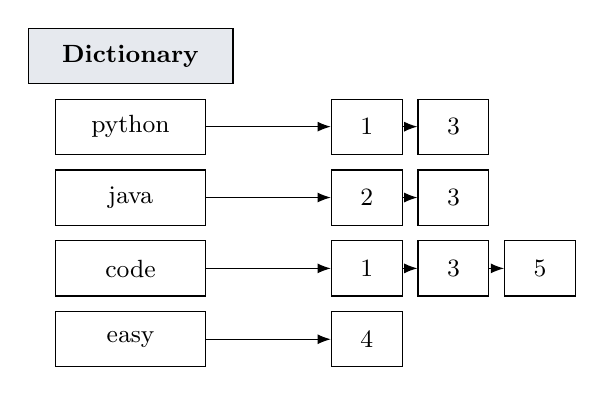
\begin{tikzpicture}[node distance=0mm, every node/.style={font=\small}]
  \node[draw, minimum width=2.6cm, minimum height=0.7cm, fill=primary!10] (d1) at (0,0) {\textbf{Dictionary}};
  \node[draw, minimum width=1.9cm, minimum height=0.7cm] (t1) at (0,-0.9) {python};
  \node[draw, minimum width=1.9cm, minimum height=0.7cm] (t2) at (0,-1.8) {java};
  \node[draw, minimum width=1.9cm, minimum height=0.7cm] (t3) at (0,-2.7) {code};
  \node[draw, minimum width=1.9cm, minimum height=0.7cm] (t4) at (0,-3.6) {easy};

  \node[draw, minimum width=0.9cm, minimum height=0.7cm] (p11) at (3.0,-0.9) {1};
  \node[draw, minimum width=0.9cm, minimum height=0.7cm] (p12) at (4.1,-0.9) {3};

  \node[draw, minimum width=0.9cm, minimum height=0.7cm] (p21) at (3.0,-1.8) {2};
  \node[draw, minimum width=0.9cm, minimum height=0.7cm] (p22) at (4.1,-1.8) {3};

  \node[draw, minimum width=0.9cm, minimum height=0.7cm] (p31) at (3.0,-2.7) {1};
  \node[draw, minimum width=0.9cm, minimum height=0.7cm] (p32) at (4.1,-2.7) {3};
  \node[draw, minimum width=0.9cm, minimum height=0.7cm] (p33) at (5.2,-2.7) {5};

  \node[draw, minimum width=0.9cm, minimum height=0.7cm] (p41) at (3.0,-3.6) {4};

  \draw[-{Latex}] (t1) -- (p11); \draw[-{Latex}] (p11) -- (p12);
  \draw[-{Latex}] (t2) -- (p21); \draw[-{Latex}] (p21) -- (p22);
  \draw[-{Latex}] (t3) -- (p31); \draw[-{Latex}] (p31) -- (p32); \draw[-{Latex}] (p32) -- (p33);
  \draw[-{Latex}] (t4) -- (p41);
\end{tikzpicture}
\end{center}
\begin{center}\small Figure 1.1: Inverted index for the corpus in Worked Example 1.1 (dictionary $\to$ sorted postings lists of docIDs).\end{center}

\subsection{Processing Boolean Queries: The Merge Algorithm}

To answer \textsf{AND} and \textsf{OR} queries efficiently, we exploit the fact that postings lists are kept \emph{sorted} by docID. Two sorted lists can be intersected or unioned in a single linear pass using two pointers.

\begin{formulabox}[Key Formula 1.1 -- Cost of the Merge Algorithm]
If two postings lists have lengths $x$ and $y$, intersecting (or unioning) them by the merge algorithm takes
\[
O(x+y)
\]
comparisons in the worst case -- each pointer only ever advances forward, and every advance is paid for by one comparison.
\end{formulabox}

\begin{algorithm}[H]
\caption{\textsc{IntersectPostings}$(p_1, p_2)$}
\begin{algorithmic}[1]
\State $answer \gets \langle\ \rangle$
\While{$p_1 \neq \textsc{nil}$ \textbf{and} $p_2 \neq \textsc{nil}$}
  \If{$docID(p_1) = docID(p_2)$}
    \State \textsc{Append}$(answer, docID(p_1))$
    \State $p_1 \gets next(p_1)$; \ $p_2 \gets next(p_2)$
  \ElsIf{$docID(p_1) < docID(p_2)$}
    \State $p_1 \gets next(p_1)$
  \Else
    \State $p_2 \gets next(p_2)$
  \EndIf
\EndWhile
\State \Return $answer$
\end{algorithmic}
\end{algorithm}

\begin{examplebox}[Worked Example 1.2 -- Merging Postings by Hand]
Using Figure 1.1, evaluate \textsf{python AND code}: postings are $\langle 1,3\rangle$ and $\langle 1,3,5\rangle$.

\begin{center}
\begin{tabular}{@{}ccccl@{}}
\toprule
Step & $p_1$ points at & $p_2$ points at & Compare & Action \\
\midrule
1 & 1 & 1 & $1=1$ & output 1; advance both \\
2 & 3 & 3 & $3=3$ & output 3; advance both \\
3 & \textsc{nil} & 5 & -- & $p_1$ exhausted, stop \\
\bottomrule
\end{tabular}
\end{center}
Result: $\langle 1,3\rangle$, found in $2$ comparisons (here $x=2,y=3$, and $2 \le x+y=5$, consistent with Key Formula 1.1).

Now evaluate \textsf{code AND NOT python}: start from $\langle 1,3,5\rangle$ (code) and remove any docID that also appears in $\langle 1,3\rangle$ (python) by the same merge logic, keeping only the elements of the first list with no match in the second: $1$ matches (drop), $3$ matches (drop), $5$ has no match in python's list (keep). Result: $\langle 5\rangle$.
\end{examplebox}

\begin{exercisebox}[Practice Exercise 1.1]
Using the postings lists of Figure 1.1 (\textsf{python}$=\langle1,3\rangle$, \textsf{java}$=\langle2,3\rangle$, \textsf{code}$=\langle1,3,5\rangle$, \textsf{easy}$=\langle4\rangle$):
\begin{enumerate}[label=(\alph*)]
  \item Compute \textsf{java OR easy} by merging, showing your pointer-walk table.
  \item Compute \textsf{python AND java} by merging.
  \item How many total comparisons did the merge in part (b) take? Confirm it does not exceed $x+y$.
\end{enumerate}
\end{exercisebox}

\Solution
\textbf{(a)} Merging $\langle2,3\rangle$ and $\langle4\rangle$ (union: keep every element, output the smaller and advance, output both and advance both on a tie): compare $2$ vs $4\Rightarrow$ output 2, advance java pointer; compare $3$ vs $4\Rightarrow$ output 3, advance java pointer; java list exhausted, flush remainder of easy list: output 4. Result: $\langle 2,3,4\rangle$.\\
\textbf{(b)} Merging $\langle1,3\rangle$ and $\langle2,3\rangle$: compare $1$ vs $2\Rightarrow$ no match, advance smaller (python); compare $3$ vs $2\Rightarrow$ no match, advance smaller (java); compare $3$ vs $3\Rightarrow$ match, output 3, advance both; both lists exhausted. Result: $\langle3\rangle$.\\
\textbf{(c)} 3 comparisons were used; $x+y = 2+2 = 4 \ge 3$. \checkmark

\subsection{Optimizing Multi-Term AND Queries}

When a query has more than two \textsf{AND}-ed terms, the \emph{order} in which postings lists are merged matters a great deal, because each intermediate result becomes the input to the next merge.

\begin{formulabox}[Key Formula 1.2 -- Greedy Merge Order]
For a query $t_1 \text{ AND } t_2 \text{ AND } \cdots \text{ AND } t_k$, process the terms in order of \textbf{increasing document frequency} $df_{t}$ (equivalently, increasing postings-list length). Always merge the current (shrinking) intermediate result with the next-shortest remaining list. This minimizes the total work because the intermediate result can never grow larger than the shortest list merged so far.
\end{formulabox}

\begin{exercisebox}[Practice Exercise 1.2]
A query engine reports the following document frequencies: $df(\textsf{database})=500$, $df(\textsf{index})=1{,}000$, $df(\textsf{query})=50$. For the query \textsf{database AND index AND query}, in what order should the three postings lists be merged? Explain using Key Formula 1.2.
\end{exercisebox}

\Solution
Sort terms by increasing $df$: \textsf{query} ($50$) $<$ \textsf{database} ($500$) $<$ \textsf{index} ($1{,}000$). So first intersect \textsf{query} and \textsf{database} (the two shortest lists), producing an intermediate result no longer than $50$ items; then intersect that result with \textsf{index}. Processing \textsf{index} first (length $1{,}000$) against another long list would waste comparisons on many docIDs that are doomed to be eliminated later.

\section{The Term Vocabulary}

Before any index can be built, raw text must be converted into a stream of index terms. This pipeline is called \textbf{tokenization and normalization}.

\subsection{Tokenization}

\begin{defbox}[Definition 1.4 -- Token, Type, Term]
A \textbf{token} is an instance of a sequence of characters in a document that is grouped together as a useful semantic unit (e.g.\ one occurrence of ``code''). A \textbf{type} is the class of all tokens with the same character sequence. A \textbf{term} is a (possibly normalized) type that is entered into the IR system's dictionary.
\end{defbox}

Tokenization raises many non-trivial decisions: should \textsf{Berkeley's} split into \textsf{Berkeley} $+$ \textsf{'s}? Should \textsf{co-education} be one token or two? Is \textsf{192.168.1.1} one token? Real systems resolve these with language- and application-specific rules; for this course, assume simple whitespace/punctuation splitting unless told otherwise.

\subsection{Stop Words}

\begin{defbox}[Definition 1.5 -- Stop Words]
\textbf{Stop words} are extremely common words (\emph{the, a, is, of, and, \ldots}) that are often \emph{excluded} from the index because they have very low discriminating power and occur in nearly every document (recall Worked Example 3.1 later, where a term occurring in \emph{every} document receives an $idf$ of exactly $0$).
\end{defbox}

Modern web search engines tend to keep stop words (indexed cheaply, e.g.\ via impact-ordered postings) because they matter for phrase queries (``to be or not to be''), but the classical exclusion technique remains important for compact indexes and for simpler classroom examples.

\subsection{Normalization and Case Folding}

\textbf{Normalization} maps superficially different tokens that should be treated as the same term into one canonical form: \textsf{U.S.A.} $\to$ \textsf{USA}, \textsf{anti-discriminatory} $\to$ \textsf{antidiscriminatory}. \textbf{Case folding} reduces all letters to lower case so that \textsf{Automobile} and \textsf{automobile} become the same term (with care taken for mid-sentence proper nouns and acronyms, e.g.\ \textsf{General Motors} vs.\ \textsf{gm}).

\subsection{Stemming and Lemmatization}
\label{sec:stemming}

\begin{defbox}[Definition 1.6 -- Stemming vs. Lemmatization]
\textbf{Stemming} crudely chops off word endings using heuristic rules to conflate related forms (\textsf{automate}, \textsf{automatic}, \textsf{automation} $\to$ \textsf{automat}). \textbf{Lemmatization} uses vocabulary and morphological analysis to return the dictionary base form, or \emph{lemma} (\textsf{is}, \textsf{was}, \textsf{be} $\to$ \textsf{be}).
\end{defbox}

The Porter stemmer is the classic English stemming algorithm, applying an ordered sequence of suffix-stripping rules (e.g.\ \textsf{SSES} $\to$ \textsf{SS}, \textsf{IES}$\to$\textsf{I}, \textsf{ATIONAL}$\to$\textsf{ATE}). For hand exercises we use a small simplified rule table capturing the flavor of Porter's algorithm without its full complexity:

\begin{center}
\begin{tabular}{@{}clll@{}}
\toprule
Rule & Condition & Suffix & Replacement \\
\midrule
S1 & word ends in & \textsf{ies} & $\to$ \textsf{y} \\
S2 & word ends in & \textsf{sses} & $\to$ \textsf{ss} \\
S3 & word ends in & \textsf{ing} (stem has a vowel) & $\to$ (drop) \\
S4 & word ends in & \textsf{ed} (stem has a vowel) & $\to$ (drop) \\
S5 & word ends in & \textsf{s} (not \textsf{ss}) & $\to$ (drop) \\
\bottomrule
\end{tabular}
\end{center}

\begin{examplebox}[Worked Example 1.3 -- Tokenize, Remove Stop Words, Stem]
Sentence: \textit{``The runners were running quickly and easily across the fields.''}

\textbf{Step 1 (tokenize \& case-fold):} the, runners, were, running, quickly, and, easily, across, the, fields

\textbf{Step 2 (remove stop words)} using stoplist \{the, were, and\}: runners, running, quickly, easily, across, fields

\textbf{Step 3 (apply stemming rules S1--S5):}
\begin{center}
\begin{tabular}{@{}lll@{}}
\toprule
Token & Rule applied & Stem \\
\midrule
runners & S5 (\textsf{s} dropped) & runner \\
running & S3 (\textsf{ing} dropped) & runn \\
quickly & none apply & quickly \\
easily & none apply & easily \\
across & none apply & across \\
fields & S5 (\textsf{s} dropped) & field \\
\bottomrule
\end{tabular}
\end{center}
\Note{\textsf{running} $\to$ \textsf{runn} rather than the ``correct'' \textsf{run} is a classic stemming over-/under-stemming artifact -- our simplified rule set does not undouble the consonant. This is exactly the kind of imprecision real stemmers like Porter's are carefully engineered to avoid, and why lemmatization is sometimes preferred when precision on word form matters.}
\end{examplebox}

\begin{exercisebox}[Practice Exercise 1.3]
Sentence: \textit{``The boxes were packed and shipped quickly by the studies team.''} Using stoplist \{the, were, and, by\} and rules S1--S5 above:
\begin{enumerate}[label=(\alph*)]
  \item Tokenize and case-fold.
  \item Remove stop words.
  \item Apply the stemming rules to each remaining token.
\end{enumerate}
\end{exercisebox}

\Solution
\textbf{(a)} the, boxes, were, packed, and, shipped, quickly, by, the, studies, team\\
\textbf{(b)} Removing \{the, were, and, by\}: boxes, packed, shipped, quickly, studies, team\\
\textbf{(c)}
\begin{center}
\begin{tabular}{@{}lll@{}}
\toprule
Token & Rule applied & Stem \\
\midrule
boxes & S5 (\textsf{s} dropped) & boxe \\
packed & S4 (\textsf{ed} dropped) & pack \\
shipped & S4 (\textsf{ed} dropped) & shipp \\
quickly & none apply & quickly \\
studies & S1 (\textsf{ies}$\to$\textsf{y}) & study \\
team & none apply & team \\
\bottomrule
\end{tabular}
\end{center}
\Note{\textsf{boxes}$\to$\textsf{boxe} and \textsf{shipped}$\to$\textsf{shipp} again show why real stemmers add extra rules (e.g., undoubling a doubled final consonant, restoring a dropped \textsf{e}); our 5-rule set is intentionally simplified for hand practice.}

% ======================================================================
% WEEK 2
% ======================================================================
\weekpart{2}{Dictionaries, Tolerant Retrieval, and Index Construction}

\section{Dictionary Data Structures}

The dictionary (vocabulary) of an inverted index must support fast lookup of a query term's postings-list pointer. Two common structures:
\begin{itemize}
  \item \textbf{Sorted array / B-tree}: enables binary search, $O(\log|V|)$ lookup, and -- crucially -- supports \emph{range} and \emph{prefix} queries (e.g., all terms between \textsf{hot} and \textsf{hotel}), which a hash table cannot.
  \item \textbf{Hash table}: $O(1)$ average lookup for a single exact term, but no support for prefix/wildcard/range queries and it must be resized as the vocabulary grows.
\end{itemize}

\section{Wildcard Queries and the Permuterm Index}

\begin{defbox}[Definition 2.1 -- Permuterm Index]
For each dictionary term $t$, append a special end-of-word symbol \$ and form all \emph{rotations} of the string $t\$$. Each rotation is stored in the dictionary pointing back to $t$. A wildcard query of the general form $X\!*\!Y$ (text $X$ before the wildcard, text $Y$ after) is answered by rotating the query itself to $Y\$X$ and doing a \emph{prefix} search for $Y\$X$ in the rotated dictionary.
\end{defbox}

\begin{examplebox}[Worked Example 2.1 -- Permuterm Rotation and Lookup]
Take the single dictionary term \textsf{money}. Form \textsf{money\$} and rotate it one character at a time:
\[
\textsf{money\$},\ \textsf{oney\$m},\ \textsf{ney\$mo},\ \textsf{ey\$mon},\ \textsf{y\$mone},\ \textsf{\$money}
\]
All six rotations are stored in the permuterm dictionary, each pointing to the original term \textsf{money}.

Now answer the wildcard query \textsf{mon*y} (matches any word starting with \textsf{mon} and ending in \textsf{y}). Rewrite $X\!*\!Y$ with $X=\textsf{mon}, Y=\textsf{y}$ as the rotated pattern $Y\$X = \textsf{y\$mon}$, and search the rotated dictionary for entries with this exact \emph{prefix}. Rotation \#5, \textsf{y\$mone}, begins with \textsf{y\$mon} -- match! It points back to \textsf{money}, which is returned.
\end{examplebox}

\begin{exercisebox}[Practice Exercise 2.1]
The dictionary contains only the term \textsf{hello}.
\begin{enumerate}[label=(\alph*)]
  \item Write out all rotations of \textsf{hello\$}.
  \item Which rotation prefix would you search to answer the wildcard query \textsf{hel*o}? Show the rewritten pattern and identify the matching rotation.
\end{enumerate}
\end{exercisebox}

\Solution
\textbf{(a)} $\textsf{hello\$},\ \textsf{ello\$h},\ \textsf{llo\$he},\ \textsf{lo\$hel},\ \textsf{o\$hell},\ \textsf{\$hello}$.\\
\textbf{(b)} Query \textsf{hel*o} has $X=\textsf{hel}$, $Y=\textsf{o}$, so we search for prefix $Y\$X=\textsf{o\$hel}$. Rotation \#5, \textsf{o\$hell}, begins with \textsf{o\$hel} -- match, pointing back to \textsf{hello}.

\Note{$k$-gram indexes are a lighter-weight alternative to permuterm indexes: every dictionary term is broken into overlapping $k$-character substrings (padded with \$ at the boundaries), and each $k$-gram points to the list of terms containing it. A wildcard query is broken into its own $k$-grams, and candidate terms are those whose $k$-gram sets have high overlap with the query's -- which is exactly the Jaccard-coefficient idea used below for spelling correction.}

\section{Spelling Correction}

\subsection{Edit Distance}

\begin{defbox}[Definition 2.2 -- Levenshtein (Edit) Distance]
The \textbf{edit distance} between two strings is the minimum number of single-character insertions, deletions, and substitutions required to transform one string into the other.
\end{defbox}

\begin{formulabox}[Key Formula 2.1 -- Edit Distance Dynamic Program]
Let $s_1$ (length $n$) and $s_2$ (length $m$) be the two strings. Define $D[i,j]$ = edit distance between the first $i$ characters of $s_1$ and the first $j$ characters of $s_2$. Then:
\[
D[i,0] = i, \qquad D[0,j] = j,
\]
\[
D[i,j] = \min \begin{cases}
D[i-1,j] + 1 & \text{(deletion)} \\
D[i,j-1] + 1 & \text{(insertion)} \\
D[i-1,j-1] + \mathbb{1}[s_1[i]\ne s_2[j]] & \text{(substitution / match)}
\end{cases}
\]
The answer is $D[n,m]$.
\end{formulabox}

\begin{examplebox}[Worked Example 2.2 -- Edit Distance by Dynamic Programming Table]
Compute the edit distance between \textsf{kitten} ($s_1$) and \textsf{sitting} ($s_2$).

\begin{center}
\begin{tabular}{@{}c|cccccccc@{}}
 & \textbf{\#} & s & i & t & t & i & n & g \\
\midrule
\textbf{\#} & 0 & 1 & 2 & 3 & 4 & 5 & 6 & 7 \\
k & 1 & 1 & 2 & 3 & 4 & 5 & 6 & 7 \\
i & 2 & 2 & 1 & 2 & 3 & 4 & 5 & 6 \\
t & 3 & 3 & 2 & 1 & 2 & 3 & 4 & 5 \\
t & 4 & 4 & 3 & 2 & 1 & 2 & 3 & 4 \\
e & 5 & 5 & 4 & 3 & 2 & 2 & 3 & 4 \\
n & 6 & 6 & 5 & 4 & 3 & 3 & 2 & 3 \\
\end{tabular}
\end{center}

Reading off $D[6,7] = 3$: three edits are needed (substitute \textsf{k}$\to$\textsf{s}, substitute \textsf{e}$\to$\textsf{i}, insert \textsf{g}), matching $\textsf{kitten} \to \textsf{sitten} \to \textsf{sittin} \to \textsf{sitting}$.

\textbf{How the last entry was filled, as a template:} $D[6,7] = \min\big(D[5,7]+1,\ D[6,6]+1,\ D[5,6]+\mathbb{1}[\textsf{n}\ne\textsf{g}]\big) = \min(4+1,\,2+1,\,3+1) = 3$ (the minimum comes from the diagonal move $D[5,6]+1$, since $\textsf{n}\ne\textsf{g}$).
\end{examplebox}

\begin{exercisebox}[Practice Exercise 2.2]
Compute the edit distance between \textsf{flaw} and \textsf{lawn} by filling in the full dynamic-programming table (rows = \textsf{flaw}, columns = \textsf{lawn}). State the minimum-cost edit sequence.
\end{exercisebox}

\Solution
\begin{center}
\begin{tabular}{@{}c|ccccc@{}}
 & \textbf{\#} & l & a & w & n \\
\midrule
\textbf{\#} & 0 & 1 & 2 & 3 & 4 \\
f & 1 & 1 & 2 & 3 & 4 \\
l & 2 & 1 & 2 & 3 & 4 \\
a & 3 & 2 & 1 & 2 & 3 \\
w & 4 & 3 & 2 & 1 & 2 \\
\end{tabular}
\end{center}
$D[4,4]=2$. Edit sequence: delete leading \textsf{f} ($\textsf{flaw}\to\textsf{law}$), then insert trailing \textsf{n} ($\textsf{law}\to\textsf{lawn}$) -- 2 edits.

\subsection{Jaccard Coefficient for $k$-gram Candidate Generation}

\begin{formulabox}[Key Formula 2.2 -- Jaccard Coefficient]
For two sets $X$ and $Y$ (here, bigram sets of two strings):
\[
J(X,Y) = \frac{|X \cap Y|}{|X \cup Y|}, \qquad 0 \le J(X,Y) \le 1.
\]
A spelling corrector uses $J$ as a cheap first filter: only dictionary terms whose $k$-gram set is sufficiently similar to the misspelled query's $k$-gram set are passed on to the (more expensive) edit-distance computation.
\end{formulabox}

\begin{examplebox}[Worked Example 2.3 -- Bigram Jaccard by Hand]
Compare \textsf{stat} and \textsf{stet} using character bigrams (no boundary padding).

Bigrams of \textsf{stat}: \textsf{st}, \textsf{ta}, \textsf{at} $\to$ set $\{\textsf{st},\textsf{ta},\textsf{at}\}$, size 3.\\
Bigrams of \textsf{stet}: \textsf{st}, \textsf{te}, \textsf{et} $\to$ set $\{\textsf{st},\textsf{te},\textsf{et}\}$, size 3.

Intersection: $\{\textsf{st}\}$, size 1. Union: $\{\textsf{st},\textsf{ta},\textsf{at},\textsf{te},\textsf{et}\}$, size 5.
\[
J(\textsf{stat},\textsf{stet}) = \frac{1}{5} = 0.2
\]
\end{examplebox}

\begin{exercisebox}[Practice Exercise 2.3]
Compute the bigram Jaccard coefficient between \textsf{night} and \textsf{nigth} (a common transposition typo).
\end{exercisebox}

\Solution
Bigrams of \textsf{night}: \textsf{ni}, \textsf{ig}, \textsf{gh}, \textsf{ht} -- set size 4.\\
Bigrams of \textsf{nigth}: \textsf{ni}, \textsf{ig}, \textsf{gt}, \textsf{th} -- set size 4.\\
Intersection: $\{\textsf{ni},\textsf{ig}\}$, size 2. Union: $\{\textsf{ni},\textsf{ig},\textsf{gh},\textsf{ht},\textsf{gt},\textsf{th}\}$, size 6.
\[
J = \frac{2}{6} = \frac{1}{3} \approx 0.333
\]

\section{Index Construction}

\subsection{Blocked Sort-Based Indexing (BSBI)}

When the collection is too large to sort all term--docID pairs in memory at once, BSBI processes the collection in blocks:

\begin{algorithm}[H]
\caption{\textsc{BSBI-Indexing}}
\begin{algorithmic}[1]
\While{documents remain}
  \State read a block of documents that fits in memory
  \State parse it into a list of (term, docID) pairs
  \State sort the pairs by term, then by docID
  \State write the sorted block to disk as a mini inverted index
\EndWhile
\State merge all the on-disk blocks (multi-way merge) into one final inverted index
\end{algorithmic}
\end{algorithm}

\subsection{Single-Pass In-Memory Indexing (SPIMI)}

SPIMI avoids ever sorting explicitly in memory: for each block, it builds postings lists incrementally in a hash table (dictionary term $\to$ growing postings list) as it streams through the tokens, then dumps the block's dictionary to disk sorted by term, and starts a fresh dictionary for the next block. This is simpler and typically faster than BSBI because there is no separate sort step over raw pairs.

\begin{examplebox}[Worked Example 2.4 -- Constructing an Inverted Index by Hand]
Mini corpus (4 documents; stop words intentionally retained here to show the raw mechanics):
\begin{center}
\begin{tabular}{@{}cl@{}}
\toprule
Doc & Text \\
\midrule
1 & the cat sat \\
2 & the dog sat on the mat \\
3 & cat and dog play \\
4 & the mat is red \\
\bottomrule
\end{tabular}
\end{center}

\textbf{Step 1 -- emit (term, docID) pairs} in document order:
\begin{center}
\small
(the,1) (cat,1) (sat,1) \ (the,2) (dog,2) (sat,2) (on,2) (the,2) (mat,2) \ (cat,3) (and,3) (dog,3) (play,3) \ (the,4) (mat,4) (is,4) (red,4)
\end{center}

\textbf{Step 2 -- sort by term, then by docID:}
\begin{center}
\small
(and,3) (cat,1) (cat,3) (dog,2) (dog,3) (is,4) (mat,2) (mat,4) (on,2) (play,3) (red,4) (sat,1) (sat,2) (the,1) (the,2) (the,2) (the,4)
\end{center}

\textbf{Step 3 -- group consecutive same-term entries into a postings list, collapsing repeated docIDs into one entry with a term frequency count:}
\begin{center}
\begin{tabular}{@{}ll@{}}
\toprule
Term & Postings (docID:freq) \\
\midrule
and & 3:1 \\
cat & 1:1, 3:1 \\
dog & 2:1, 3:1 \\
is & 4:1 \\
mat & 2:1, 4:1 \\
on & 2:1 \\
play & 3:1 \\
red & 4:1 \\
sat & 1:1, 2:1 \\
the & 1:1, 2:\textbf{2}, 4:1 \\
\bottomrule
\end{tabular}
\end{center}
Notice \textsf{the} occurs \emph{twice} within document 2 (``\textit{the} dog sat on \textit{the} mat''), so the two (the,2) pairs collapse into a single postings entry \textsf{2:2} recording term frequency 2, rather than two separate entries.
\end{examplebox}

\begin{exercisebox}[Practice Exercise 2.4]
Build the inverted index (postings with term-frequency counts) for this 3-document corpus by hand, following the same three steps:
\begin{center}
\begin{tabular}{@{}cl@{}}
\toprule
Doc & Text \\
\midrule
1 & fox jumps over the fox \\
2 & the dog sleeps \\
3 & fox and dog run \\
\bottomrule
\end{tabular}
\end{center}
\end{exercisebox}

\Solution
Term--docID pairs: (fox,1)(jumps,1)(over,1)(the,1)(fox,1) $\to$ (the,2)(dog,2)(sleeps,2) $\to$ (fox,3)(and,3)(dog,3)(run,3).\\
Sorted: (and,3)(dog,2)(dog,3)(fox,1)(fox,1)(fox,3)(jumps,1)(over,1)(run,3)(sleeps,2)(the,1)(the,2).\\
Grouped postings:
\begin{center}
\begin{tabular}{@{}ll@{}}
\toprule
Term & Postings (docID:freq) \\
\midrule
and & 3:1 \\
dog & 2:1, 3:1 \\
fox & 1:\textbf{2}, 3:1 \\
jumps & 1:1 \\
over & 1:1 \\
run & 3:1 \\
sleeps & 2:1 \\
the & 1:1, 2:1 \\
\bottomrule
\end{tabular}
\end{center}
(\textsf{fox} appears twice in document 1, collapsing to \textsf{1:2}.)

\subsection{Distributed and Dynamic Indexing (Conceptual Overview)}

\begin{itemize}
  \item \textbf{Distributed indexing (MapReduce)}: \emph{parsers} (mappers) split the collection into (term, docID) pairs; the pair space is partitioned by term range across machines; \emph{inverters} (reducers) collect all pairs for their assigned term range and write sorted postings -- BSBI's block-and-merge idea, parallelized across a cluster.
  \item \textbf{Dynamic indexing}: new documents cannot cheaply be inserted into one giant sorted index. The standard solution keeps a small, easily-rebuilt \textbf{auxiliary index} in memory for recent documents, answers queries against \emph{both} the main and auxiliary index, and periodically \textbf{merges} the auxiliary index into the main index (logarithmic merging schedules multiple auxiliary indexes of geometrically increasing size to bound the total re-merging cost).
\end{itemize}



% ======================================================================
% WEEK 3
% ======================================================================
\weekpart{3}{Term Weighting, the Vector Space Model, and Efficient Scoring}

\section{Parametric and Zone Indexes}

Real documents have structure beyond a flat bag of words: a \textbf{title}, an \textbf{author} field, a \textbf{date}, an \textbf{abstract}. A \textbf{parametric index} lets a query restrict on such fields directly (e.g., \textsf{date} $=2023$). A \textbf{zone} is a named region of free text within a document (title, body, anchor text); a \textbf{zone index} keeps a separate postings list per zone so that a match in the title can be treated differently from a match in the body -- the basis of \emph{weighted zone scoring} in Section~\ref{sec:zone-scoring}.

\section{Term Frequency and Document Frequency}

\begin{defbox}[Definition 3.1 -- tf and df]
The \textbf{term frequency} $tf_{t,d}$ is the raw count of term $t$ in document $d$. The \textbf{document frequency} $df_t$ is the number of documents in the collection containing $t$ at least once (not to be confused with the \emph{collection frequency}, the total count of $t$ over all documents).
\end{defbox}

Raw $tf$ is a poor weight on its own: a document with $tf=20$ is not ``20 times as relevant'' as one with $tf=1$. IR systems therefore commonly \textbf{dampen} $tf$, e.g.\ with a log transform $wf_{t,d} = 1+\log(tf_{t,d})$ for $tf_{t,d}>0$ (and $0$ otherwise).

\subsection{Inverse Document Frequency}

\begin{formulabox}[Key Formula 3.1 -- Inverse Document Frequency]
\[
idf_t = \log\!\left(\frac{N}{df_t}\right)
\]
where $N$ is the total number of documents in the collection. A term in \emph{every} document has $df_t=N$, so $idf_t = \log(1) = 0$ -- it is given \emph{no} weight at all, formalizing the intuition behind stop-word removal (Definition 1.5).
\end{formulabox}

\Note{Any logarithm base may be used ($2$, $10$, $e$); changing the base multiplies every $idf_t$ (and hence every $tf\text{-}idf$ weight) by the same constant $\log_b(a)$, so relative rankings by cosine similarity are completely unaffected. In the worked examples below we deliberately use $\log_2$ with a collection size that is a power of $2$, purely so the arithmetic can be done without a calculator.}

\subsection{tf-idf Weighting}
\label{sec:vsm-tfidf}

\begin{formulabox}[Key Formula 3.2 -- tf-idf Weight]
\[
tf\text{-}idf_{t,d} \;=\; tf_{t,d} \times idf_t
\]
This single number is high when $t$ occurs often in $d$ (informative about $d$) \emph{and} $t$ is rare across the collection (informative in general) -- and low whenever either factor is low.
\end{formulabox}

\begin{examplebox}[Worked Example 3.1 -- Computing $idf$ and tf-idf with Clean Numbers]
Collection size $N=8$. Vocabulary of interest: \textsf{the}, \textsf{internet}, \textsf{protocol}, \textsf{network}, with document frequencies $df(\textsf{the})=8$, $df(\textsf{internet})=4$, $df(\textsf{protocol})=2$, $df(\textsf{network})=1$.

\[
idf(\textsf{the}) = \log_2\tfrac{8}{8} = \log_2 1 = 0, \qquad
idf(\textsf{internet}) = \log_2\tfrac{8}{4} = \log_2 2 = 1,
\]
\[
idf(\textsf{protocol}) = \log_2\tfrac{8}{2} = \log_2 4 = 2, \qquad
idf(\textsf{network}) = \log_2\tfrac{8}{1} = \log_2 8 = 3.
\]

Document $D_3$ has raw counts $tf(\textsf{the})=10$, $tf(\textsf{internet})=4$, $tf(\textsf{protocol})=2$, $tf(\textsf{network})=1$. Then:
\[
tf\text{-}idf(\textsf{the},D_3) = 10\times 0 = 0, \qquad tf\text{-}idf(\textsf{internet},D_3)=4\times1=4,
\]
\[
tf\text{-}idf(\textsf{protocol},D_3)=2\times2=4, \qquad tf\text{-}idf(\textsf{network},D_3)=1\times3=3.
\]
So $D_3$'s tf-idf vector, in the order (the, internet, protocol, network), is $(0,4,4,3)$.
\end{examplebox}

\begin{exercisebox}[Practice Exercise 3.1]
Using the same $idf$ values as Worked Example 3.1, document $D_2$ has raw counts $tf(\textsf{the})=8$, $tf(\textsf{internet})=2$, $tf(\textsf{protocol})=0$, $tf(\textsf{network})=2$. Compute $D_2$'s full tf-idf vector.
\end{exercisebox}

\Solution
$tf\text{-}idf(\textsf{the},D_2)=8\times0=0$; $tf\text{-}idf(\textsf{internet},D_2)=2\times1=2$; $tf\text{-}idf(\textsf{protocol},D_2)=0\times2=0$; $tf\text{-}idf(\textsf{network},D_2)=2\times3=6$.\\
$D_2 = (0,2,0,6)$.

\section{The Vector Space Model}

\begin{defbox}[Definition 3.2 -- Vector Space Model (VSM)]
Each document $d$ (and the query $q$) is represented as a vector in $\mathbb{R}^{|V|}$, one dimension per vocabulary term, with the tf-idf weight as the coordinate. Similarity between $q$ and $d$ is measured as the \textbf{cosine} of the angle between their vectors -- \emph{not} their Euclidean distance, because cosine similarity is insensitive to document length (a long document that repeats the same topic should not automatically win just because its raw vector is longer).
\end{defbox}

\begin{formulabox}[Key Formula 3.3 -- Cosine Similarity]
\[
\cos(\vec q, \vec d) \;=\; \frac{\vec q \cdot \vec d}{\lVert \vec q\rVert\,\lVert \vec d\rVert} \;=\; \frac{\sum_{t} q_t\, d_t}{\sqrt{\sum_t q_t^2}\;\sqrt{\sum_t d_t^2}}
\]
Equivalently: normalize $\vec q$ and $\vec d$ to unit vectors first, then take their dot product.
\end{formulabox}

\begin{examplebox}[Worked Example 3.2 -- Cosine Similarity Intuition in 2 Dimensions]
Let $D_1=(4,0)$, $D_2=(0,3)$, query $Q=(2,1)$.
\[
\lVert D_1\rVert = 4, \quad \lVert D_2\rVert = 3, \quad \lVert Q\rVert = \sqrt{2^2+1^2}=\sqrt5 \approx 2.236
\]
\[
\cos(Q,D_1) = \frac{2(4)+1(0)}{4\times2.236} = \frac{8}{8.944} \approx 0.894
\]
\[
\cos(Q,D_2) = \frac{2(0)+1(3)}{3\times2.236} = \frac{3}{6.708} \approx 0.447
\]
$D_1$ ranks above $D_2$: its direction is closer to $Q$'s, even though we never computed a Euclidean distance.
\end{examplebox}

\begin{examplebox}[Worked Example 3.3 -- Full tf-idf + Cosine Ranking]
Reuse $idf(\textsf{the})=0, idf(\textsf{internet})=1, idf(\textsf{protocol})=2, idf(\textsf{network})=3$ and $D_2=(0,2,0,6)$, $D_3=(0,4,4,3)$ from above, and add $D_1$ with raw counts $tf(\textsf{the})=5,tf(\textsf{protocol})=3$ (internet, network absent), giving $D_1 = (5\times0,\ 0,\ 3\times2,\ 0) = (0,0,6,0)$.

Query: ``\textsf{protocol network}'' -- raw query term count $1$ each, weighted by $idf$: $Q = (0,\,0,\,1\times2,\,1\times3) = (0,0,2,3)$.

\textbf{Norms:}
\[
\lVert D_1\rVert=\sqrt{6^2}=6,\quad \lVert D_2\rVert=\sqrt{2^2+6^2}=\sqrt{40}\approx6.325,\quad \lVert D_3\rVert=\sqrt{4^2+4^2+3^2}=\sqrt{41}\approx6.403,
\]
\[
\lVert Q\rVert = \sqrt{2^2+3^2}=\sqrt{13}\approx3.606.
\]

\textbf{Dot products:}
\[
Q\cdot D_1 = 2(6)+3(0)=12, \qquad Q\cdot D_2 = 2(0)+3(6)=18, \qquad Q\cdot D_3 = 2(4)+3(3)=17.
\]

\textbf{Cosine similarities:}
\[
\cos(Q,D_1)=\frac{12}{6\times3.606}=\frac{12}{21.63}\approx0.555,
\]
\[
\cos(Q,D_2)=\frac{18}{6.325\times3.606}=\frac{18}{22.81}\approx0.789,
\]
\[
\cos(Q,D_3)=\frac{17}{6.403\times3.606}=\frac{17}{23.09}\approx0.736.
\]

\textbf{Ranking:} $D_2\ (0.789) \;>\; D_3\ (0.736) \;>\; D_1\ (0.555)$.
\end{examplebox}

\Note{$D_2$ ranks \emph{above} $D_3$ even though $D_2$ has \emph{zero} weight on \textsf{protocol} while $D_3$ matches both query terms! Cosine similarity depends on the overall \emph{direction} of the document vector, not simply on how many query terms it contains -- $D_2$'s very high weight on \textsf{network} (idf $=3$) dominates the dot product and gives it a slightly larger numerator relative to its norm. This is a genuine, well-known property of the vector space model, not an error.}

\begin{exercisebox}[Practice Exercise 3.2]
Using the same three document vectors $D_1=(0,0,6,0)$, $D_2=(0,2,0,6)$, $D_3=(0,4,4,3)$ (order: the, internet, protocol, network), re-rank them for the query ``\textsf{internet protocol}'', i.e.\ $Q=(0,\,1\times1,\,1\times2,\,0)=(0,1,2,0)$. Compute all three cosine similarities and give the final ranking.
\end{exercisebox}

\Solution
$\lVert Q\rVert=\sqrt{1^2+2^2}=\sqrt5\approx2.236$.\\
$Q\cdot D_1 = 1(0)+2(6)=12$; $\ \cos(Q,D_1)=\dfrac{12}{6\times2.236}=\dfrac{12}{13.42}\approx0.894$.\\
$Q\cdot D_2 = 1(2)+2(0)=2$; $\ \cos(Q,D_2)=\dfrac{2}{6.325\times2.236}=\dfrac{2}{14.14}\approx0.141$.\\
$Q\cdot D_3 = 1(4)+2(4)=12$; $\ \cos(Q,D_3)=\dfrac{12}{6.403\times2.236}=\dfrac{12}{14.32}\approx0.838$.\\
\textbf{Ranking:} $D_1\ (0.894) \;>\; D_3\ (0.838) \;>\; D_2\ (0.141)$. (Here $D_2$ drops to last, since it has no weight on \textsf{protocol} and only a small \textsf{internet} weight relative to its large \textsf{network}-dominated norm.)

\section{Efficient Scoring}
\label{sec:zone-scoring}

Computing full cosine similarity against every document in the collection is wasteful when only a handful of documents can possibly score well. Real systems use several tricks:

\begin{itemize}
  \item \textbf{Document-at-a-time scoring}: iterate through postings lists in parallel by increasing docID, accumulating each document's full score before moving to the next docID (requires all postings sorted by docID -- exactly the structure used for Boolean merging in Week 1).
  \item \textbf{Term-at-a-time scoring}: process one query term's entire postings list at a time, accumulating partial scores per document in an accumulator array, then move to the next term. Simpler to reason about, but needs an accumulator per candidate document.
  \item \textbf{Tiered indexes / champion lists}: keep a short list of the highest-$tf\text{-}idf$ documents for each term (a ``champion list''); try to satisfy the query from these small lists first, only falling back to the full postings lists if too few results are found.
\end{itemize}

\subsection{Weighted Zone Scoring}

\begin{formulabox}[Key Formula 3.4 -- Weighted Zone Scoring]
Given $\ell$ zones with weights $g_1,\dots,g_\ell$ (typically $\sum_i g_i = 1$) and a Boolean match indicator $s_i \in \{0,1\}$ for each zone (does the query term/expression match in zone $i$?):
\[
\text{score} = \sum_{i=1}^{\ell} g_i\, s_i
\]
\end{formulabox}

\begin{exercisebox}[Practice Exercise 3.3]
A search engine uses two zones, title (weight $g_{\text{title}}=0.6$) and body (weight $g_{\text{body}}=0.4$), for the query term \textsf{java}. Three documents match as follows: $D_1$ (title only), $D_2$ (body only), $D_3$ (both title and body). Rank $D_1,D_2,D_3$ by weighted zone score.
\end{exercisebox}

\Solution
$\text{score}(D_1) = 0.6(1)+0.4(0) = 0.6$; $\ \text{score}(D_2)=0.6(0)+0.4(1)=0.4$; $\ \text{score}(D_3)=0.6(1)+0.4(1)=1.0$.\\
Ranking: $D_3\ (1.0) > D_1\ (0.6) > D_2\ (0.4)$.

\subsection{The BM25 Scoring Function}

BM25 (``Best Match 25'') is the classic probabilistically-motivated scoring function used as the industry-standard baseline ranking function, refining raw tf-idf with document-length normalization.

\begin{formulabox}[Key Formula 3.5 -- Okapi BM25]
\[
\text{score}(D,Q) = \sum_{t \in Q} idf(t)\cdot \frac{f(t,D)\,(k_1+1)}{f(t,D) + k_1\left(1-b+b\dfrac{|D|}{\text{avgdl}}\right)}
\]
where $f(t,D)$ is the raw term frequency of $t$ in $D$, $|D|$ is the length of $D$, $\text{avgdl}$ is the average document length in the collection, and $idf(t) = \ln\!\dfrac{N-df_t+0.5}{df_t+0.5}$. The free parameters $k_1$ (typically $\approx1.2$) control term-frequency saturation, and $b$ (typically $0.75$) controls the strength of length normalization.
\end{formulabox}

\Note{As $f(t,D)\to\infty$, the term's contribution saturates at $idf(t)\cdot(k_1+1)$ rather than growing without bound as raw tf-idf would -- this is the key mathematical improvement BM25 makes over Key Formula 3.2.}

\begin{examplebox}[Worked Example 3.4 -- Computing a BM25 Score]
Collection: $N=10$, $\text{avgdl}=50$, $k_1=1.2$, $b=0.75$. Query terms \textsf{network} ($df=2$) and \textsf{protocol} ($df=3$). Document $D$ has $|D|=60$, $f(\textsf{network},D)=3$, $f(\textsf{protocol},D)=1$.

\textbf{Step 1 -- idf:}
\[
idf(\textsf{network}) = \ln\frac{10-2+0.5}{2+0.5} = \ln\frac{8.5}{2.5}=\ln 3.4 \approx 1.2238
\]
\[
idf(\textsf{protocol}) = \ln\frac{10-3+0.5}{3+0.5} = \ln\frac{7.5}{3.5}=\ln 2.1429 \approx 0.7621
\]

\textbf{Step 2 -- length-normalization factor} (same for every term in this document):
\[
1-b+b\frac{|D|}{\text{avgdl}} = 1-0.75+0.75\times\frac{60}{50} = 0.25+0.9=1.15, \qquad k_1\times1.15 = 1.38
\]

\textbf{Step 3 -- per-term score:}
\[
\textsf{network}: \ \frac{3(1.2+1)}{3+1.38}=\frac{6.6}{4.38}\approx1.5068 \ \Rightarrow\ 1.2238\times1.5068\approx1.8441
\]
\[
\textsf{protocol}: \ \frac{1(2.2)}{1+1.38}=\frac{2.2}{2.38}\approx0.9244 \ \Rightarrow\ 0.7621\times0.9244\approx0.7045
\]

\textbf{Step 4 -- total:}
\[
\text{score}(D,Q) = 1.8441+0.7045 \approx 2.5486
\]
\end{examplebox}

\begin{exercisebox}[Practice Exercise 3.4]
Using the same collection statistics and $idf$ values as Worked Example 3.4 ($idf(\textsf{network})\approx1.2238$, $idf(\textsf{protocol})\approx0.7621$, $k_1=1.2$, $b=0.75$, $\text{avgdl}=50$), a different document $D'$ has $|D'|=40$, $f(\textsf{network},D')=1$, $f(\textsf{protocol},D')=2$. Compute $\text{score}(D',Q)$.
\end{exercisebox}

\Solution
Length factor: $1-0.75+0.75\times\dfrac{40}{50}=0.25+0.6=0.85$; \ $k_1\times0.85=1.02$.\\
\textsf{network} ($f=1$): $\dfrac{1(2.2)}{1+1.02}=\dfrac{2.2}{2.02}\approx1.0891 \Rightarrow 1.2238\times1.0891\approx1.3330$.\\
\textsf{protocol} ($f=2$): $\dfrac{2(2.2)}{2+1.02}=\dfrac{4.4}{3.02}\approx1.4570 \Rightarrow 0.7621\times1.4570\approx1.1103$.\\
\textbf{Total:} $\text{score}(D',Q) \approx 1.3330+1.1103 = 2.4433$.

% ======================================================================
% WEEK 4
% ======================================================================
\weekpart{4}{Evaluation, Relevance Feedback, and Query Expansion}

\section{Evaluating an Unranked Retrieval Set}

\begin{defbox}[Definition 4.1 -- Precision and Recall]
Given a query, a system's returned set, and a ground-truth relevance judgment, define:
$TP$ = relevant \& retrieved, $FP$ = non-relevant \& retrieved, $FN$ = relevant \& not retrieved.
\[
\text{Precision } P = \frac{TP}{TP+FP}, \qquad \text{Recall } R = \frac{TP}{TP+FN}
\]
\end{defbox}

\begin{formulabox}[Key Formula 4.1 -- $F_1$ Measure]
\[
F_1 = \frac{2PR}{P+R}
\]
the harmonic mean of precision and recall -- chosen over the arithmetic mean because it penalizes a system that scores very low on \emph{either} $P$ or $R$ much more heavily.
\end{formulabox}

\begin{examplebox}[Worked Example 4.1 -- Precision, Recall, $F_1$ from a Contingency Table]
A collection has $10$ documents relevant to a query. A system retrieves $8$ documents, of which $5$ are relevant.
\[
TP=5,\quad FP=8-5=3,\quad FN=10-5=5
\]
\[
P=\frac{5}{5+3}=\frac{5}{8}=0.625, \qquad R=\frac{5}{5+5}=\frac{5}{10}=0.5
\]
\[
F_1 = \frac{2(0.625)(0.5)}{0.625+0.5} = \frac{0.625}{1.125} \approx 0.5556
\]
\end{examplebox}

\begin{exercisebox}[Practice Exercise 4.1]
A collection has $12$ documents relevant to a query. A system retrieves $9$ documents, of which $6$ are relevant. Compute $P$, $R$, and $F_1$.
\end{exercisebox}

\Solution
$TP=6$, $FP=9-6=3$, $FN=12-6=6$.\ \ $P=\dfrac{6}{9}\approx0.667$, \ $R=\dfrac{6}{12}=0.5$.\\
$F_1 = \dfrac{2(0.667)(0.5)}{0.667+0.5}=\dfrac{0.667}{1.167}\approx0.5715$.

\section{Evaluating a Ranked Retrieval List}

\subsection{Average Precision and Mean Average Precision}

\begin{formulabox}[Key Formula 4.2 -- Average Precision (AP)]
For one query with $R$ total relevant documents in the collection, let $P(k)$ be the precision computed at the rank $k$ of each successive relevant document retrieved (documents never retrieved contribute $0$):
\[
AP = \frac{1}{R}\sum_{\text{relevant } d}\ P(\text{rank of } d)
\]
\textbf{Mean Average Precision (MAP)} is the mean of $AP$ over a set of queries:
\[
MAP = \frac{1}{|Q|}\sum_{q\in Q} AP(q)
\]
\end{formulabox}

\begin{examplebox}[Worked Example 4.2 -- Computing AP and MAP]
\textbf{Query 1:} $6$ total relevant documents exist. The ranked results (R = relevant, N = not) are:
\[
\underbrace{R}_{1}\ \underbrace{N}_{2}\ \underbrace{R}_{3}\ \underbrace{R}_{4}\ \underbrace{N}_{5}\ \underbrace{N}_{6}\ \underbrace{R}_{7}\ \underbrace{N}_{8}\ \underbrace{N}_{9}\ \underbrace{R}_{10}
\]
Precision at each relevant rank: $P(1)=\tfrac11=1.0$, $P(3)=\tfrac23\approx0.667$, $P(4)=\tfrac34=0.75$, $P(7)=\tfrac47\approx0.571$, $P(10)=\tfrac5{10}=0.5$. Only $5$ of the $6$ relevant documents were retrieved at all, so the $6^{\text{th}}$ contributes $0$.
\[
AP_1 = \frac{1.0+0.667+0.75+0.571+0.5+0}{6} = \frac{3.488}{6} \approx 0.5814
\]

\textbf{Query 2:} $2$ total relevant documents, ranked results: $N\ R\ R\ N\ N$.
$P(2)=\tfrac12=0.5$, $P(3)=\tfrac23\approx0.667$.
\[
AP_2 = \frac{0.5+0.667}{2} = \frac{1.167}{2} \approx 0.5835
\]

\[
MAP = \frac{AP_1+AP_2}{2} = \frac{0.5814+0.5835}{2}\approx 0.5824
\]
\end{examplebox}

\begin{exercisebox}[Practice Exercise 4.2]
A query has $4$ total relevant documents. The ranked results are: $R\ R\ N\ N\ R\ N$ (all $3$ relevant documents that exist among these six ranks were retrieved, but a $4^{\text{th}}$ relevant document elsewhere in the collection was never retrieved). Compute $AP$ for this query.
\end{exercisebox}

\Solution
$P(1)=\tfrac11=1.0$, $P(2)=\tfrac22=1.0$, $P(5)=\tfrac35=0.6$; the $4^{\text{th}}$ relevant document contributes $0$.
\[
AP = \frac{1.0+1.0+0.6+0}{4} = \frac{2.6}{4} = 0.65
\]

\subsection{Normalized Discounted Cumulative Gain (nDCG)}

\begin{formulabox}[Key Formula 4.3 -- DCG and nDCG]
With graded relevance scores $rel_1, rel_2, \dots, rel_p$ at ranks $1,\dots,p$:
\[
DCG_p = rel_1 + \sum_{i=2}^{p} \frac{rel_i}{\log_2 i}
\]
$IDCG_p$ is $DCG_p$ computed on the \emph{ideal} ranking (relevance scores sorted in descending order). Then:
\[
nDCG_p = \frac{DCG_p}{IDCG_p} \in [0,1]
\]
\end{formulabox}

\begin{center}
\small \textit{Useful values:} $\log_2 2=1$, $\log_2 3\approx1.585$, $\log_2 4=2$, $\log_2 5\approx2.322$, $\log_2 6\approx2.585$
\end{center}

\begin{examplebox}[Worked Example 4.3 -- Computing nDCG]
Ranked list of $5$ documents with graded relevance $rel = [3,2,3,0,1]$.

\textbf{Actual DCG:}
\[
DCG_5 = 3 + \frac{2}{\log_2 2} + \frac{3}{\log_2 3} + \frac{0}{\log_2 4} + \frac{1}{\log_2 5}
= 3 + \frac{2}{1} + \frac{3}{1.585} + \frac{0}{2} + \frac{1}{2.322}
\]
\[
= 3 + 2 + 1.893 + 0 + 0.431 = 7.324
\]

\textbf{Ideal ranking} (sort relevance descending): $[3,3,2,1,0]$.
\[
IDCG_5 = 3 + \frac{3}{1} + \frac{2}{1.585} + \frac{1}{2} + \frac{0}{2.322} = 3+3+1.262+0.5+0 = 7.762
\]

\[
nDCG_5 = \frac{7.324}{7.762} \approx 0.9436
\]
\end{examplebox}

\begin{exercisebox}[Practice Exercise 4.3]
Ranked list of $6$ documents with graded relevance $rel = [2,3,2,0,1,2]$. Compute $DCG_6$, $IDCG_6$, and $nDCG_6$.
\end{exercisebox}

\Solution
\[
DCG_6 = 2 + \frac{3}{\log_22} + \frac{2}{\log_23} + \frac{0}{\log_24} + \frac{1}{\log_25} + \frac{2}{\log_26}
= 2+3+\frac{2}{1.585}+0+\frac{1}{2.322}+\frac{2}{2.585}
\]
\[
= 2+3+1.262+0+0.431+0.774 = 7.467
\]
Ideal order (descending): $[3,2,2,2,1,0]$.
\[
IDCG_6 = 3+\frac{2}{1}+\frac{2}{1.585}+\frac{2}{2}+\frac{1}{2.322}+\frac{0}{2.585} = 3+2+1.262+1+0.431+0 = 7.693
\]
\[
nDCG_6 = \frac{7.467}{7.693} \approx 0.9706
\]

\section{Relevance Feedback: The Rocchio Algorithm}

\begin{defbox}[Definition 4.2 -- Relevance Feedback]
After an initial query, the user marks some returned documents \emph{relevant} and others \emph{non-relevant}. The system uses these judgments to build an improved query and re-run the search -- without the user ever typing a new query.
\end{defbox}

\begin{formulabox}[Key Formula 4.4 -- Rocchio's Formula]
\[
\vec q_m = \alpha\, \vec q_0 \;+\; \beta\,\frac{1}{|D_r|}\sum_{\vec d \in D_r} \vec d \;-\; \gamma\,\frac{1}{|D_{nr}|}\sum_{\vec d \in D_{nr}} \vec d
\]
where $\vec q_0$ is the original query vector, $D_r$ and $D_{nr}$ are the sets of documents (as tf-idf vectors) marked relevant and non-relevant, and $\alpha,\beta,\gamma \ge 0$ trade off trust in the original query versus the feedback (common published defaults: $\alpha=1,\ \beta=0.75,\ \gamma=0.15$; we use $\gamma=0.25$ below purely to keep the hand-arithmetic clean).
\end{formulabox}

\begin{examplebox}[Worked Example 4.4 -- Rocchio Update by Hand]
$\vec q_0 = (1,0,1)$. One relevant document $\vec d_1=(1,1,0)$, one non-relevant document $\vec d_2=(0,1,1)$. Use $\alpha=1,\beta=0.75,\gamma=0.25$.

Since there is only one document in each set, the ``mean'' is just that document itself:
\[
\vec q_m = 1\cdot(1,0,1) + 0.75\cdot(1,1,0) - 0.25\cdot(0,1,1)
\]
\[
= (1,0,1) + (0.75,0.75,0) - (0,0.25,0.25) = (1+0.75-0,\ 0+0.75-0.25,\ 1+0-0.25)
\]
\[
\vec q_m = (1.75,\ 0.5,\ 0.75)
\]
Notice the weight on dimension 2 rose from $0$ to $0.5$ (pulled toward the relevant document) while dimension 3 fell from $1$ to $0.75$ (pushed away from the non-relevant document, which also had a $1$ there).
\end{examplebox}

\begin{exercisebox}[Practice Exercise 4.4]
$\vec q_0=(0,1,1)$. Two relevant documents $\vec d_1=(1,1,0)$ and $\vec d_2=(1,0,1)$; one non-relevant document $\vec d_3=(0,0,1)$. Using $\alpha=1,\beta=0.75,\gamma=0.25$, compute $\vec q_m$. (Remember $D_r$'s contribution uses the \emph{mean} of $\vec d_1,\vec d_2$.)
\end{exercisebox}

\Solution
Mean of relevant set: $\dfrac{(1,1,0)+(1,0,1)}{2} = (1,\,0.5,\,0.5)$.
\[
\vec q_m = 1\cdot(0,1,1) + 0.75\cdot(1,0.5,0.5) - 0.25\cdot(0,0,1)
\]
\[
= (0,1,1)+(0.75,0.375,0.375)-(0,0,0.25) = (0.75,\ 1.375,\ 1.125)
\]

\section{Probabilistic Relevance Feedback (Preview)}

Vector-space (Rocchio) feedback moves the \emph{query vector} toward relevant documents and away from non-relevant ones -- a purely geometric operation. \textbf{Probabilistic} relevance feedback instead updates the \emph{term-weight statistics} themselves: for each query term $t$, the counts of how often $t$ appears in the (now-judged) relevant vs.\ non-relevant documents are refined, and a new probabilistic weight (Key Formula 5.1, Week 5) is recomputed from these updated counts. The two approaches are compared directly in Section~\ref{sec:vsm-vs-prob} once the probabilistic model has been introduced.

\section{Query Expansion}

\begin{defbox}[Definition 4.3 -- Query Expansion]
\textbf{Query expansion} adds new terms to a query, either from a hand-built \textbf{thesaurus} (e.g., automatically adding \textsf{automobile} when the user types \textsf{car}) or from an \textbf{automatically derived} thesaurus built by clustering terms that co-occur frequently in the same documents or the same local context windows across the collection.
\end{defbox}

Query expansion and relevance feedback solve the same underlying problem -- the user's original keywords are an imperfect proxy for their information need -- but query expansion modifies the query \emph{before} seeing any results (using global collection statistics), whereas relevance feedback modifies it \emph{after} seeing which specific documents the user judged relevant.

% ======================================================================
% WEEK 5
% ======================================================================
\weekpart{5}{Probabilistic Information Retrieval and Language Models for IR}

\section{The Probability Ranking Principle}

\begin{defbox}[Definition 5.1 -- Probability Ranking Principle (PRP)]
If documents are ranked in decreasing order of their probability of relevance to the query, $P(R=1\mid d,q)$, given all the evidence available, then the overall effectiveness of the system to its users is the best obtainable.
\end{defbox}

The PRP is the theoretical justification for \emph{every} ranking function in this course: tf-idf/cosine, BM25, and language-model scores are all, in different ways, attempts to \emph{approximate} $P(R=1\mid d,q)$.

\subsection{Intuition: The PRP as a Decision Problem}

The PRP can feel like a tautology -- ``to get the best results, show the most likely relevant things first'' -- but behind this statement is a precise decision-theoretic argument, proposed by Stephen Robertson in 1977.

\textbf{Analogy.} Suppose a doctor has 5 candidate medicines for a patient, each taking 1 hour to administer, tried one at a time: medicine A has an 80\% chance of curing the patient, B has 50\%, and C has 10\%. To minimize the patient's expected suffering, the doctor should try them in decreasing order of success probability: $A \to B \to C$. A search engine faces the same problem -- the user's attention is limited, and every document shown carries some probability of satisfying the need ($R=1$) or wasting the user's time ($R=0$).

\textbf{Proof sketch (cost framework).} For a document $d$, let $P(R=1\mid d)$ be its probability of relevance and $P(R=0\mid d) = 1-P(R=1\mid d)$. Define two costs: $C_1$, the cost of showing a non-relevant document, and $C_0$, the cost of omitting or delaying a relevant one. The expected cost of presenting $d$ is
\[
EC(d) = C_1\,P(R=0\mid d) - C_0\,P(R=1\mid d) = C_1 - (C_1+C_0)\,P(R=1\mid d).
\]
Preferring $d_1$ over $d_2$ whenever $EC(d_1) < EC(d_2)$ and substituting the expression above, the $C_1$ terms cancel and dividing by $-(C_1+C_0)$ (flipping the inequality) gives
\[
P(R=1\mid d_1) > P(R=1\mid d_2).
\]
So minimizing expected cost is equivalent to ranking documents by decreasing $P(R=1\mid d)$ -- exactly the PRP.

\textbf{Hidden assumptions (why PRP breaks in practice).}
\begin{itemize}
\item \textbf{Independent relevance:} $P(R=1\mid d_1)$ is assumed independent of $d_2$. If $d_1$ is a comprehensive guide and $d_2$ is an exact duplicate, $d_2$ still has high $P(R=1)$ and PRP ranks it second -- but to the user, $d_2$ now has zero marginal utility, since they already read $d_1$.
\item \textbf{Binary utility:} documents are treated as strictly relevant or non-relevant, ignoring degree of relevance, freshness, diversity, or ambiguity in user intent.
\end{itemize}
\section{The Binary Independence Model (BIM)}

The BIM operationalizes the PRP: it gives a concrete, computable estimate of $P(R=1\mid d,q)$ by making two strict simplifying assumptions.

\begin{defbox}[Definition 5.2 -- Binary Independence Model]
\textbf{Binary document representation:} a document $D$ is represented as a binary incidence vector $\vec{x} = (x_1,\dots,x_V) \in \{0,1\}^V$ over the vocabulary, where $x_t=1$ if term $t$ is present and $x_t=0$ if absent (as in Week 1's incidence matrix). Term frequency and document length are ignored entirely.

\textbf{Conditional independence:} terms are assumed to occur \emph{independently of one another} within the set of relevant documents ($R=1$), and independently within the set of non-relevant documents ($R=0$). This is a strong assumption -- real terms co-occur -- but it is exactly what makes the model tractable.
\end{defbox}

\subsection{The $2\times2$ Contingency Table}

For a single query term $t$, define over the whole judged collection: $N$ = total documents, $R$ = total relevant documents, $n_t$ = documents containing $t$, $r_t$ = relevant documents containing $t$. This gives the following $2\times2$ contingency table:

\begin{center}
\begin{tabular}{@{}lccc@{}}
\toprule
 & Relevant Docs ($R=1$) & Non-Relevant Docs ($R=0$) & Row Totals \\
\midrule
Contains Word $t$ & $r_t$ (Hits) & $n_t - r_t$ (False Alarms) & $n_t$ (All docs with word) \\
Missing Word $t$  & $R - r_t$ (Misses) & $(N - n_t) - (R - r_t)$ (True Negatives) & $N - n_t$ (All docs without word) \\
\midrule
Column Totals & $R$ (Total relevant) & $N-R$ (Total non-relevant) & $N$ (Total collection size) \\
\bottomrule
\end{tabular}
\end{center}

\begin{formulabox}[Key Formula 5.1 -- RSJ (Robertson--Sparck Jones) Term Weight]
Define the term occurrence probabilities
\[
p_t = P(x_t=1\mid R=1) = \frac{r_t}{R}, \qquad u_t = P(x_t=1\mid R=0) = \frac{n_t-r_t}{N-R}.
\]
The retrieval status value contributed by matching term $t$ is
\[
c_t = \log_2 \frac{p_t(1-u_t)}{u_t(1-p_t)}.
\]
Substituting the raw contingency-table counts for $p_t$ and $u_t$ gives the equivalent count-only form
\[
c_t = \log_2 \frac{r_t \cdot \big[(N-R) - (n_t - r_t)\big]}{(n_t - r_t)\cdot(R - r_t)} = \log_2 \frac{r_t \,(N - R - n_t + r_t)}{(n_t - r_t)\,(R - r_t)}.
\]
A document's overall score (its \emph{retrieval status value}) is the sum of $c_t$ over all query terms $t$ that it contains:
\[
RSV(D) = \sum_{t \,\in\, Q \cap D} c_t.
\]
Larger $c_t$ means $t$ is a much better discriminator of relevance (much more likely in relevant than non-relevant documents).
\end{formulabox}

\subsection{Intuition: Topic vs.\ Word}

The variables in the contingency table are easy to confuse because they mix two different notions: $R$ is about the \emph{topic} the user actually wants, while $n_t$ and $r_t$ are about a \emph{specific word} $t$ used to search for it. A document can be relevant to the topic without containing the word, and it can contain the word without being relevant to the topic.

\textbf{Analogy.} Suppose the search topic is ``Heart Disease'' and the search word is $t=$ ``cholesterol,'' over a collection of $N=1000$ medical documents.
\begin{itemize}
\item $N = 1000$ -- the entire document collection.
\item $R = 25$ -- documents actually \emph{about} heart disease. A document can be about heart disease without ever using the word ``cholesterol'' (it might discuss ``heart attacks,'' ``stents,'' or ``blood pressure'' instead).
\item $n_t = 50$ -- documents anywhere in the collection that contain the word ``cholesterol.'' Some of these may be dietary guides or biology textbooks that have nothing to do with heart disease.
\item $r_t = 20$ -- the \emph{overlap}: of the 25 heart-disease documents, 20 happen to mention ``cholesterol.''
\item $R - r_t = 5$ -- relevant documents that \emph{missed} the word (they discuss heart disease using other terms).
\item $n_t - r_t = 30$ -- non-relevant documents that \emph{happen to contain} the word (nutrition blogs, gallstone articles, etc.).
\end{itemize}

\begin{center}
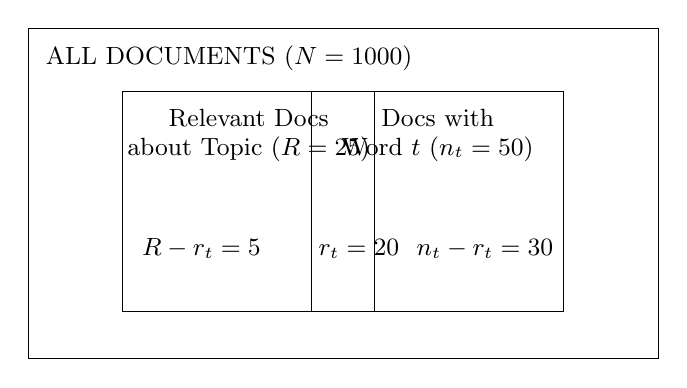
\begin{tikzpicture}[font=\small]
\draw (0,0) rectangle (8,4.2);
\node[anchor=north west] at (0.1,4.1) {ALL DOCUMENTS ($N=1000$)};
\draw (1.2,0.6) rectangle (4.4,3.4);
\node[anchor=north] at (2.8,3.3) {Relevant Docs};
\node[anchor=north] at (2.8,2.95) {about Topic ($R=25$)};
\draw (3.6,0.6) rectangle (6.8,3.4);
\node[anchor=north] at (5.2,3.3) {Docs with};
\node[anchor=north] at (5.2,2.95) {Word $t$ ($n_t=50$)};
\node at (2.2,1.4) {$R - r_t = 5$};
\node at (4.2,1.4) {$r_t = 20$};
\node at (5.8,1.4) {$n_t - r_t = 30$};
\end{tikzpicture}
\end{center}

\begin{examplebox}[Worked Example 5.1 -- Computing an RSJ Term Weight]
Collection: $N=1000$ documents, $R=25$ documents judged relevant to a query. Term $t$ appears in $n_t=50$ documents total, of which $r_t=20$ are relevant.

\textbf{Step 1 -- populate the contingency table.}
\begin{center}
\begin{tabular}{@{}lccc@{}}
\toprule
 & Relevant Docs ($R=25$) & Non-Relevant Docs ($N-R=975$) & Row Totals \\
\midrule
Contains Word $t$ & $r_t = 20$ (Hits) & $n_t - r_t = 30$ (False Alarms) & $n_t = 50$ \\
Missing Word $t$  & $R - r_t = 5$ (Misses) & $(1000-50)-5 = 945$ (True Negatives) & $N-n_t = 950$ \\
\midrule
Column Totals & $R=25$ & $N-R=975$ & $N=1000$ \\
\bottomrule
\end{tabular}
\end{center}

\textbf{Step 2 -- occurrence probabilities.}
\[
p_t = \frac{r_t}{R} = \frac{20}{25} = 0.8, \qquad 1-p_t = 0.2
\]
\[
u_t = \frac{n_t-r_t}{N-R} = \frac{50-20}{1000-25} = \frac{30}{975} \approx 0.03077, \qquad 1-u_t \approx 0.96923
\]

\textbf{Step 3 -- RSJ weight, via probabilities.}
\[
c_t = \log_2 \frac{0.8\times0.96923}{0.03077\times0.2} = \log_2\frac{0.77538}{0.006154} = \log_2(126.0) \approx 6.977 \text{ bits}
\]

\textbf{Verification -- direct count substitution.} Using the count-only form of Key Formula 5.1 gives the same result without computing $p_t$ and $u_t$ explicitly:
\[
c_t = \log_2 \frac{r_t\,(N-R-n_t+r_t)}{(n_t-r_t)(R-r_t)} = \log_2\frac{20 \times (1000-25-50+20)}{(50-20)\times(25-20)} = \log_2\frac{20\times945}{30\times5} = \log_2\frac{18900}{150} = \log_2(126) \approx 6.977 \text{ bits}
\]
A document containing this single term $t$ would receive a document score of $\approx6.98$.
\end{examplebox}

\begin{exercisebox}[Practice Exercise 5.1]
Collection: $N=2000$, $R=40$. Term $t$ appears in $n_t=80$ documents, of which $r_t=30$ are relevant. Compute $p_t$, $u_t$, and $c_t$ (base 2).
\end{exercisebox}

\Solution
\[
p_t = \frac{30}{40} = 0.75, \qquad u_t = \frac{80-30}{2000-40} = \frac{50}{1960} \approx 0.02551
\]
\[
c_t = \log_2\frac{0.75\times0.97449}{0.02551\times0.25} = \log_2\frac{0.73087}{0.006378} = \log_2(114.6) \approx 6.84 \text{ bits}
\]

\subsection{Query vs.\ Information Need: Where Do $R$, $p_t$, and $u_t$ Come From?}

Key Formula 5.1 assumes $R$ and $r_t$ are already known -- but this hides the central dilemma of IR: the gap between a \textbf{query} and an \textbf{information need}.

\begin{defbox}[Definition 5.3 -- Query vs.\ Information Need]
The \textbf{information need} is the user's actual underlying intention (e.g., ``I want to understand heart disease, its causes, and treatments''), which exists only in the user's head. The \textbf{query} is the imperfect proxy the user types (e.g., $t=$ ``cholesterol''). A document is defined as relevant ($R=1$) if it satisfies the information need, regardless of the exact words it uses -- but the system observes only the query term $t$, never the need itself.
\end{defbox}

\textbf{Real-world analogy.} Returning to the ``Heart Disease'' / ``cholesterol'' example: the user's information need is ``I want to understand heart disease, its causes, and treatments,'' but all the system ever receives is the query term $t=$ ``cholesterol.'' The system does not read the user's mind -- it has no way to directly observe which of its $N=1000$ documents belong to the true relevant set $R=25$. All it can see, at query time, is $n_t=50$: how many documents happen to contain the word ``cholesterol.'' The true overlap $r_t=20$ is exactly the quantity the system \emph{cannot} know in advance -- it depends on the user's underlying intention, not on any word count. This is the catch-22: if $R$ (and hence $r_t$, $p_t$, $u_t$) depends on subjective intention the system cannot observe, how can it rank documents by Key Formula 5.1 at all before showing any results? In practice, probabilistic search engines resolve this in two stages.

\textbf{Stage A -- the first pass (before anything is known about $R$).} With zero relevance judgments, the system falls back on two default assumptions:
\begin{itemize}
\item $p_t \approx 0.5$: term $t$ is assumed equally likely to appear or not appear in a relevant document (an uninformative prior).
\item $u_t \approx n_t/N$: since the collection $N$ is huge and the (unknown) relevant set $R$ is tiny by comparison, the non-relevant set is approximated by the \emph{entire} collection.
\end{itemize}
Substituting these into Key Formula 5.1:
\[
c_t \approx \log_2 \frac{0.5\,(1-n_t/N)}{(n_t/N)\,(1-0.5)} = \log_2\frac{1-n_t/N}{n_t/N} \approx \log_2\frac{N}{n_t} \quad \text{when } n_t \ll N,
\]
which is exactly the \textbf{IDF (Inverse Document Frequency)} term weight. So on the very first pass -- before any relevance information exists -- the RSJ model degenerates to ranking purely by term rarity, which is precisely why tf-idf/BM25-style IDF weighting is theoretically justified as an approximation to $c_t$ under total ignorance of $R$. In the cholesterol example, the system's very first ranking would simply use $c_t \approx \log_2(1000/50) = \log_2(20) \approx 4.32$ bits -- no knowledge of the true 25 heart-disease documents is needed or used yet.

\textbf{Stage B -- relevance feedback (once $R$ becomes observable).} Once initial results are shown, the system can estimate $R$ and $r_t$ in one of two ways, and then recompute $p_t$, $u_t$, and $c_t$ from Key Formula 5.1 directly:
\begin{itemize}
\item \textbf{Explicit/implicit feedback:} the user clicks on (or dwells on) a handful of documents, which the system treats as newly observed members of $R$. In the analogy, suppose the user clicks on 25 documents while researching heart disease, and the system notices 20 of them contain ``cholesterol'' -- it has now directly observed $R=25$, $r_t=20$, recovering the exact contingency table used in Worked Example 5.1, and can re-rank the remaining documents with the full RSJ formula ($c_t\approx6.98$ bits) instead of the IDF guess.
\item \textbf{Pseudo-relevance feedback (PRF):} the system \emph{assumes} the top-$k$ documents from the first pass (e.g., the top 10) are relevant, sets $R=k$, counts $r_t$ within just those $k$ documents, and uses the refined weights for an automatic second retrieval pass -- without ever asking the user for real judgments. Here, the system might simply take its top 10 IDF-ranked ``cholesterol'' documents, assume all 10 are about heart disease, count how many of them actually are, and refine $c_t$ from that automatically-guessed table.
\end{itemize}

\begin{center}
\begin{tabular}{@{}p{3.2cm}p{3.4cm}p{5.4cm}@{}}
\toprule
Situation & Does the system know $R$? & Formula used \\
\midrule
Initial query & No (assumes $R$ is small and unobserved) & IDF approximation, $c_t \approx \log_2(N/n_t)$ \\
After clicks / PRF & Yes (estimated from clicked or top-$k$ docs) & Full RSJ formula, $c_t = \log_2\frac{p_t(1-u_t)}{u_t(1-p_t)}$ \\
\bottomrule
\end{tabular}
\end{center}

This is also why the \emph{probabilistic relevance feedback} discussed next is not a separate, unrelated technique -- it is simply Stage B of the BIM: the same RSJ machinery, applied once $r_t$ and $R$ can finally be measured.

\subsection{How BIM Search Works: A Step-by-Step Algorithm}

Putting Stages A and B together, a BIM-based search engine runs the following pipeline. Steps 1--4 are the \textbf{initial pass} (no relevance judgments exist yet); steps 5--8 are the \textbf{update cycle}, triggered once feedback becomes available.

\begin{defbox}[Algorithm 5.1 -- BIM Matching and Feedback Cycle]
\textbf{Phase 1 -- Initial Pass}
\begin{enumerate}
\item \textbf{Query parsing and token extraction.} The engine receives the user's query and breaks it into a set of unique search terms $Q = \{t_1, t_2, \dots, t_k\}$.
\item \textbf{Default parameter assignment.} With no relevance judgments yet available for this query, the system falls back on the Stage A default assumptions: $p_t = 0.5$ (a term is assumed equally likely to appear or not in an unknown relevant document) and $u_t \approx n_t/N$ (the term's overall collection frequency stands in for its rate in non-relevant documents).
\item \textbf{First-pass term weighting.} With $p_t=0.5$, Key Formula 5.1 collapses to the IDF form:
\[
c_t \approx \log_2 \frac{N - n_t}{n_t}.
\]
\item \textbf{Document scoring and initial ranking.} For every document, the system sums the weights of its matching query terms, $RSV(D) = \sum_{t\,\in\,Q\cap D} c_t$, sorts documents in decreasing order of $RSV$, and returns the top $K$ to the user.
\end{enumerate}

\textbf{Phase 2 -- Update Cycle}
\begin{enumerate}
\setcounter{enumi}{4}
\item \textbf{Capturing relevance feedback.} $R$ and $r_t$ are obtained either from \emph{explicit/implicit feedback} (the user clicks, views, or marks specific documents as useful) or from \emph{pseudo-relevance feedback (PRF)}, where the system simply assumes the top-10 documents from Phase 1 are relevant. Either way, the system now has $R$ = number of identified relevant documents, and $r_t$ = how many of them contain term $t$.
\item \textbf{Re-estimating $p_t$ and $u_t$.} The default assumptions are replaced by empirical estimates from the newly observed counts, typically with $+0.5$ smoothing to avoid division by zero when $r_t=0$ or $r_t=R$:
\[
p_t = \frac{r_t + 0.5}{R + 1.0}, \qquad u_t = \frac{n_t - r_t + 0.5}{N - R + 1.0}.
\]
\item \textbf{Recalculating full RSJ weights.} The system recomputes $c_t$ with the full Key Formula 5.1, $c_t = \log_2\frac{p_t(1-u_t)}{u_t(1-p_t)}$. Terms that appear in nearly all identified relevant documents ($r_t \approx R$) receive a large weight boost; terms concentrated in non-relevant documents receive low or negative weights.
\item \textbf{Re-scoring and re-ranking.} $RSV(D)$ is recomputed for every document in the collection using the updated $c_t$ values, and the results are re-ranked. Documents missed in Phase 1 -- because they lacked terms that scored well under plain IDF -- can now rise to the top if they contain terms whose $c_t$ was boosted by feedback.
\end{enumerate}
\end{defbox}

Steps 5--8 can repeat: each new round of feedback (explicit or pseudo) re-triggers Step 5, giving the system another round of refined $p_t$, $u_t$, and $c_t$ estimates.

\section{Probabilistic Relevance Feedback}
\label{sec:vsm-vs-prob}

Once a user has judged some retrieved documents relevant/non-relevant, the contingency-table counts $r_t$ and $n_t$ for every query term can be \emph{re-estimated} directly from those judgments, and the RSJ weight $c_t$ recomputed with Key Formula 5.1 -- this is probabilistic relevance feedback.

\begin{defbox}[Definition 5.3 -- Vector Space vs.\ Probabilistic Relevance Feedback]
\textbf{Rocchio (vector space) feedback}, Key Formula 4.4, is a purely \emph{geometric} operation: it nudges the query vector's coordinates toward the centroid of relevant documents and away from non-relevant ones, in the tf-idf vector space. It has no explicit probabilistic interpretation -- $\beta$ and $\gamma$ are tuned empirically, not derived from a model of relevance.\\[4pt]
\textbf{Probabilistic (BIM) feedback} re-estimates the \emph{parameters of an explicit generative model of relevance} ($p_t$ and $u_t$ for every term) directly from the judged documents, using Key Formula 5.1. The weight update is a direct consequence of Bayesian updating, not a geometric heuristic.
\end{defbox}

\begin{center}
\begin{tabular}{@{}p{3.4cm}p{5.6cm}p{5.6cm}@{}}
\toprule
 & \textbf{Vector space (Rocchio)} & \textbf{Probabilistic (BIM)} \\
\midrule
What is updated & Query vector coordinates & Per-term probabilities $p_t,u_t$ \\
Theoretical grounding & Heuristic / geometric & Probability Ranking Principle \\
Uses non-relevant docs how & Subtracts their (weighted) vector & Updates $u_t$ (false-positive rate) \\
New terms discovered via & Any term with nonzero weight in $D_r$ & Any term whose $n_t,r_t$ can be counted \\
\bottomrule
\end{tabular}
\end{center}

\section{Language Models for Information Retrieval}

Before deep learning, the language modeling approach to IR (pioneered by Ponte and Croft in 1998) offered a different way to think about ranking altogether. Rather than hand-crafting a weighting scheme like TF-IDF and asking ``how well does this document match the query,'' it turns the question around: \emph{for each document $d$, how likely is it that $d$'s own writer would have generated exactly this query $q$?} Concretely, we build for every document $d$ a \textbf{unigram language model} $M_d$ -- a probability distribution over vocabulary terms estimated purely from $d$'s own text -- and then rank documents by $P(q\mid M_d)$, the probability that $M_d$ would emit the query as output. Intuitively: which document ``sounds like'' it was written by someone who would also write this query? This reframes retrieval as a generative, probabilistic estimation problem, giving ranking a principled foundation instead of relying on ad-hoc heuristics.

\subsection{From MLE to the Zero-Probability Problem}

The natural starting point for $M_d$ is the maximum-likelihood estimate (MLE): the probability of a term $t$ under $d$'s language model is just its relative frequency in $d$,
\[
P_{\text{mle}}(t \mid d) = \frac{tf_{t,d}}{|d|}.
\]
Assuming each query term is generated independently (the unigram assumption), the probability of the whole query is the product of the per-term probabilities:
\[
P(q \mid M_d) = \prod_{i=1}^{|q|} P(q_i \mid M_d).
\]
This is elegant, but it breaks immediately in practice. A document is a short, finite sample of text, so it is normal for $d$ to simply never contain some term $t$ that appears in the query -- not because $t$ is irrelevant to $d$'s topic, but because $d$ happened not to use that particular word. The MLE estimate then assigns $P_{\text{mle}}(t\mid d) = 0$ to that term, and because the query probability is a \textbf{product} over all query terms, a single missing term drags the \emph{entire} product to zero, however well $d$ matches every other word in the query. Left uncorrected, this would make the model unusable: nearly every document would score $P(q\mid d)=0$, and ranking would collapse to only the rare documents containing every query term verbatim.

\subsection{Smoothing: Borrowing from the Collection}

The fix is \textbf{smoothing}: instead of trusting $d$'s own (sparse) word counts alone, we blend them with a \textbf{background model} $P(t\mid C)$ estimated from the whole collection $C$. The intuition is that even if $d$ never used the word ``mouse,'' the collection as a whole tells us ``mouse'' is a perfectly ordinary word with some nonzero background probability, and a well-smoothed document model should inherit a small amount of that mass rather than flatly forbidding the term. Smoothing therefore does two things at once: it repairs the zero-probability problem, and -- as a side effect -- it discounts the probability mass given to frequent terms that carry little discriminating power (much like IDF does for TF-IDF), since common terms already have high background probability and gain comparatively little from appearing in $d$.

\subsection{Jelinek--Mercer Smoothing}

The simplest and most direct way to blend the two estimates is \textbf{linear interpolation}, known as Jelinek--Mercer (JM) smoothing:
\[
P_{JM}(t\mid d) = (1-\lambda)\,P_{\text{mle}}(t\mid d) \;+\; \lambda\, P(t\mid C),
\]
where $\lambda\in[0,1]$ is a single mixing parameter controlling how much weight is shifted from the document's own statistics to the collection background. When $\lambda=0$, JM smoothing reduces exactly to the raw (and fragile) MLE estimate; as $\lambda\to1$, the document model is dominated by the collection and stops discriminating between documents at all. In between, every term -- whether it occurs in $d$ or not -- receives a nonzero probability, because $P(t\mid C)>0$ for any term that appears anywhere in the collection. The query likelihood under this smoothed model is simply the product of the smoothed per-term probabilities,
\[
P(q\mid d) = \prod_{t\in q} P_{JM}(t\mid d),
\]
and it is this quantity, not the raw MLE product, that is used to rank documents.

\begin{examplebox}[Worked Example 5.2 -- Query Likelihood with Jelinek--Mercer Smoothing]
Vocabulary $\{\textsf{cat},\textsf{dog},\textsf{mouse}\}$. Document $d$: ``\textsf{cat cat dog}'', so $|d|=3$, $tf(\textsf{cat},d)=2$, $tf(\textsf{dog},d)=1$, $tf(\textsf{mouse},d)=0$.

Collection background probabilities (estimated from the whole corpus): $P(\textsf{cat}\mid C)=0.2$, $P(\textsf{dog}\mid C)=0.3$, $P(\textsf{mouse}\mid C)=0.1$.

Query $q = $ ``\textsf{cat mouse}''. Use $\lambda=0.4$.

\textbf{MLE estimates:} $P_{\text{mle}}(\textsf{cat}\mid d)=\tfrac23\approx0.667$; $\ P_{\text{mle}}(\textsf{mouse}\mid d) = \tfrac03 = 0$.

\textbf{Smoothed estimates:}
\[
P_{JM}(\textsf{cat}\mid d) = 0.6\times0.667 + 0.4\times0.2 = 0.400+0.080 = 0.480
\]
\[
P_{JM}(\textsf{mouse}\mid d) = 0.6\times0 + 0.4\times0.1 = 0+0.040 = 0.040
\]
\[
P(q\mid d) = P_{JM}(\textsf{cat}\mid d)\times P_{JM}(\textsf{mouse}\mid d) = 0.480 \times 0.040 = 0.0192
\]
Note that without smoothing, $P(q\mid d)$ would have been exactly $0$ (because \textsf{mouse} never occurs in $d$) -- smoothing is what makes the model usable at all.
\end{examplebox}

\subsection{Dirichlet Smoothing}

Jelinek--Mercer's $\lambda$ is a single fixed knob: it mixes in the \emph{same proportion} of background probability regardless of whether $d$ is a two-word snippet or a ten-thousand-word article. That is an odd assumption -- a short document's MLE estimate is inherently noisier and deserves heavier smoothing, while a long document's own word counts are already fairly reliable and should be trusted more. \textbf{Dirichlet-prior smoothing} fixes this by smoothing not with a fixed weight but with a fixed \emph{pseudo-count} of extra, collection-flavored word occurrences added to every document, letting the effective mixing proportion adapt automatically to $d$'s length.

Concretely, imagine augmenting $d$ with $\mu$ additional word occurrences, drawn according to the background distribution $P(t\mid C)$, before computing the MLE estimate on this enlarged pseudo-document. The count of term $t$ becomes $tf_{t,d} + \mu\,P(t\mid C)$ and the total length becomes $|d|+\mu$, giving:
\[
P_{\text{Dir}}(t\mid d) = \frac{tf_{t,d} + \mu\, P(t\mid C)}{|d| + \mu},
\]
where $\mu$ is the single free parameter controlling how many ``extra'' background occurrences are injected. Rewriting this as an interpolation makes the length-adaptive behavior explicit:
\[
P_{\text{Dir}}(t\mid d) = \frac{|d|}{|d|+\mu}\,P_{\text{mle}}(t\mid d) \;+\; \frac{\mu}{|d|+\mu}\,P(t\mid C),
\]
which has exactly the same linear-interpolation shape as Jelinek--Mercer, except the effective mixing weight $\mu/(|d|+\mu)$ now shrinks as $|d|$ grows: since $\mu$ is a constant while $|d|$ varies from document to document, short documents automatically receive a large dose of smoothing (their sparse counts are barely trustworthy) and long documents receive very little (their own statistics already dominate) -- entirely without hand-tuning $\lambda$ per document length, as a fixed-$\lambda$ JM model would require.

\begin{exercisebox}[Practice Exercise 5.2]
Using the same document $d$ (\textsf{cat cat dog}, $|d|=3$) and background probabilities as Worked Example 5.2, apply \textbf{Dirichlet smoothing with $\mu=5$} instead of Jelinek--Mercer, and recompute $P(q\mid d)$ for $q=$ ``\textsf{cat mouse}''.
\end{exercisebox}

\Solution
\[
P_{\text{Dir}}(\textsf{cat}\mid d) = \frac{2 + 5(0.2)}{3+5} = \frac{2+1}{8} = \frac{3}{8} = 0.375
\]
\[
P_{\text{Dir}}(\textsf{mouse}\mid d) = \frac{0 + 5(0.1)}{3+5} = \frac{0.5}{8} = 0.0625
\]
\[
P(q\mid d) = 0.375 \times 0.0625 = 0.02344
\]

\Note{Comparing the two smoothing methods on the identical document and query: $P_{JM}(q\mid d)=0.0192$ vs.\ $P_{\text{Dir}}(q\mid d)=0.02344$ -- different smoothing methods produce different absolute probabilities, which is expected (they encode different smoothing assumptions); only the \emph{ranking} across documents needs to be sensible, not the absolute magnitude.}

\section{Neural Language Models and Dense Retrieval}

Classical language models for IR -- even smoothed ones -- are still fundamentally counting words: two documents that describe the same idea using different vocabulary (``car'' vs.\ ``automobile'') look unrelated to a unigram model, because $P(t\mid d)$ only ever assigns mass to terms that literally occur in $d$. The deep learning revolution attacked this at the representation level: instead of a discrete distribution over vocabulary terms, every query and document is mapped to a \textbf{continuous dense vector} in a learned embedding space, where semantic similarity between texts becomes geometric closeness between vectors -- regardless of whether the exact same words were used.

\begin{defbox}[Definition 5.5 -- Contextual Embeddings from Pre-trained Transformers]
Pre-trained transformer encoders (BERT, RoBERTa, and their successors) learn, from massive unlabeled text, contextual representations in which a word's vector depends on the surrounding sentence rather than being fixed in isolation. Fine-tuning these encoders for retrieval yields representations where semantically related but lexically different terms -- e.g., ``car'' and ``automobile'' -- end up close together in vector space, directly solving the \textbf{vocabulary mismatch problem} that plagues purely term-based models like TF-IDF or classical query likelihood.
\end{defbox}

Turning contextual embeddings into a working retrieval system, however, still requires deciding \emph{how} a query and a document are compared, and here two architectures make fundamentally different speed/accuracy trade-offs.

\begin{defbox}[Definition 5.6 -- Bi-Encoders (Dense Retrieval)]
A bi-encoder passes the query and the document through the transformer \textbf{independently}, each producing its own fixed-size dense vector, with no cross-attention between the two texts. Relevance is then just a similarity score between the two vectors -- cosine similarity or inner product. Because document vectors can be computed once, offline, and indexed for \textbf{approximate nearest neighbor (ANN) search}, a bi-encoder can retrieve from millions of documents in milliseconds at query time. Models such as \textbf{DPR} (Dense Passage Retrieval) and \textbf{Contriever} follow this design, making bi-encoders the workhorse of first-stage dense retrieval, playing the same role dense TF-IDF/BM25 retrieval played in classical IR.
\end{defbox}

\begin{defbox}[Definition 5.7 -- Cross-Encoders]
A cross-encoder instead feeds the query and document \textbf{together} as a single input, letting every attention layer of the transformer directly relate query tokens to document tokens before producing one relevance score. This joint attention captures fine-grained interactions a bi-encoder's independent vectors cannot, making cross-encoders substantially more accurate -- but the score cannot be precomputed, since it depends on the specific query-document pair, so every candidate document requires a full forward pass through the transformer at query time. This is far too expensive to run over an entire collection.
\end{defbox}

\begin{formulabox}[Key Insight 5.1 -- The Standard Two-Stage Pipeline]
Because bi-encoders are fast but less precise, and cross-encoders are precise but slow, modern dense retrieval systems combine them in a \textbf{retrieve-then-rerank} pipeline: a bi-encoder first retrieves a broad candidate set (e.g., top-$1000$) from the full collection via cheap ANN search, and a cross-encoder then \textbf{reranks} only that small candidate set (e.g., top-$100$) to produce the final, accurate ordering. This mirrors the classical IR pattern of a cheap first-stage ranker (BM25) followed by a more expensive learning-to-rank reranker, but with transformer encoders in both roles.
\end{formulabox}

\section{Large Language Models for IR (LLM4IR) and Retrieval-Augmented Generation}

The most recent shift is that large language models no longer sit only at the end of the pipeline as a generator of prose -- they are now woven into essentially every stage of the retrieval process itself, from reformulating the query to ranking candidates to producing the final answer grounded in retrieved evidence.

\begin{center}
\begin{tabular}{@{}p{3.6cm}p{9.4cm}@{}}
\toprule
\textbf{Pipeline Stage} & \textbf{Role of Language Models / LLMs} \\
\midrule
Query Rewriting / Expansion & Expanding short, ambiguous queries; rewriting multi-turn conversational queries into a standalone search query; or generating a \textbf{pseudo-document} that answers the query and using \emph{that} as the search vector (HyDE -- Hypothetical Document Embeddings). \\
Indexing / Retrieval & \textbf{Model-based search}, e.g.\ a Differentiable Search Index (DSI), where a single generative LM is trained to directly output a relevant document's ID as text, collapsing the index and the retriever into one model. \\
Reranking & Zero-shot or few-shot prompting of an LLM to judge and reorder top candidates by subtle contextual relevance that shallow lexical or even bi-encoder similarity scores miss. \\
Generation (RAG) & Grounding the LLM's generated response in the top-retrieved passages, so the model synthesizes an answer from actual evidence rather than relying purely on its parametric memory -- reducing hallucination and enabling up-to-date, source-attributable answers. \\
\bottomrule
\end{tabular}
\end{center}

\begin{defbox}[Definition 5.8 -- Retrieval-Augmented Generation (RAG)]
RAG couples a retriever (classical, dense, or hybrid) with a generative LLM: given a user query, the retriever fetches the top-$k$ most relevant passages from an external corpus, and these passages are inserted into the LLM's prompt as context alongside the query. The LLM then generates its answer conditioned on this retrieved evidence rather than on its training data alone. This lets a general-purpose LLM answer questions about private, proprietary, or rapidly changing information without retraining the model itself, and it gives the answer a traceable evidentiary basis -- the very same goal that motivated ranked retrieval in Week 1, now serving generation instead of a ranked list.
\end{defbox}

% ======================================================================
% WEEK 6
% ======================================================================
\weekpart{6}{Text Classification and Na\"ive Bayes}

\section{The Text Classification Problem}

\begin{defbox}[Definition 6.1 -- Text Classification]
Given a fixed set of classes $\mathbb{C} = \{c_1,\dots,c_J\}$ and a \textbf{training set} of documents each pre-labeled with a class, learn a classifier that assigns the correct class to a \textbf{new, unseen} document. This is \emph{supervised} learning, in contrast to the unsupervised indexing/ranking methods of Weeks 1--5.
\end{defbox}

Text classification underlies spam filtering, sentiment analysis, language identification, and (as we will see in Week 7) parts of web search quality control.

\section{The Naive Bayes Generative Model}

\begin{defbox}[Definition 6.2 -- Multinomial Na\"ive Bayes]
Naive Bayes models each document as generated by: (1) picking a class $c$ with probability $P(c)$, then (2) generating each word position independently from $c$'s own word distribution $P(t\mid c)$. Two independence assumptions make this tractable and give the model its name:
\begin{itemize}
  \item \textbf{Conditional independence}: the presence of one word does not affect the probability of another, given the class.
  \item \textbf{Positional independence}: $P(t\mid c)$ does not depend on a word's position in the document.
\end{itemize}
Both assumptions are literally false for real text -- yet the resulting classifier is simple, fast, and surprisingly effective.
\end{defbox}

\begin{formulabox}[Key Formula 6.1 -- MAP Classification Rule]
\[
c_{\text{map}} = \arg\max_{c \in \mathbb{C}} \; P(c) \prod_{t \in d} P(t\mid c)^{\,tf_{t,d}}
\]
(equivalently, working in log space to avoid numeric underflow: $\arg\max_c \big[\log P(c) + \sum_{t\in d} tf_{t,d}\log P(t\mid c)\big]$).
\end{formulabox}

\begin{formulabox}[Key Formula 6.2 -- Parameter Estimation with Add-One (Laplace) Smoothing]
\[
\hat P(c) = \frac{N_c}{N}, \qquad
\hat P(t\mid c) = \frac{T_{ct}+1}{\left(\sum_{t'\in V} T_{ct'}\right) + |V|}
\]
where $N_c$ is the number of training documents in class $c$, $N$ is the total number of training documents, $T_{ct}$ is the number of occurrences of term $t$ in training documents of class $c$, and $|V|$ is the vocabulary size. Add-one smoothing is essential: without it, any term never seen in class $c$'s training data would force $P(t\mid c)=0$, which would zero out the \emph{entire} product for any test document containing that term -- exactly the zero-probability problem of Key Formula 5.2.
\end{formulabox}

\begin{examplebox}[Worked Example 6.1 -- The Classic China/Japan Na\"ive Bayes Example]
Training set (class $c=$ ``China'', class $j=$ ``not-China''):

\begin{center}
\begin{tabular}{@{}clc@{}}
\toprule
Doc & Text & Class \\
\midrule
1 & Chinese Beijing Chinese & $c$ \\
2 & Chinese Chinese Shanghai & $c$ \\
3 & Chinese Macao & $c$ \\
4 & Tokyo Japan Chinese & $j$ \\
\bottomrule
\end{tabular}
\end{center}

\textbf{Test document 5:} ``Chinese Chinese Chinese Tokyo Japan'' -- classify it.

Vocabulary $V=\{\textsf{Chinese},\textsf{Beijing},\textsf{Shanghai},\textsf{Macao},\textsf{Tokyo},\textsf{Japan}\}$, $|V|=6$.

\textbf{Priors:} $N=4$ training docs, $N_c=3$, $N_j=1$.
\[
\hat P(c) = \frac34 = 0.75, \qquad \hat P(j) = \frac14 = 0.25
\]

\textbf{Class $c$ token counts} (docs 1--3, total length $8$): $\textsf{Chinese}=5$, $\textsf{Beijing}=1$, $\textsf{Shanghai}=1$, $\textsf{Macao}=1$, $\textsf{Tokyo}=0$, $\textsf{Japan}=0$.
\[
\hat P(\textsf{Chinese}\mid c) = \frac{5+1}{8+6} = \frac{6}{14} = \frac37, \qquad
\hat P(\textsf{Tokyo}\mid c) = \hat P(\textsf{Japan}\mid c) = \frac{0+1}{8+6}=\frac{1}{14}
\]

\textbf{Class $j$ token counts} (doc 4, total length $3$): $\textsf{Chinese}=1$, $\textsf{Tokyo}=1$, $\textsf{Japan}=1$.
\[
\hat P(\textsf{Chinese}\mid j) = \frac{1+1}{3+6}=\frac29, \qquad
\hat P(\textsf{Tokyo}\mid j) = \hat P(\textsf{Japan}\mid j) = \frac{1+1}{3+6}=\frac29
\]

\textbf{Score the test document} (Chinese$\times3$, Tokyo$\times1$, Japan$\times1$):
\[
\text{Score}(c) = \hat P(c)\cdot\hat P(\textsf{Chinese}\mid c)^3\cdot \hat P(\textsf{Tokyo}\mid c)\cdot\hat P(\textsf{Japan}\mid c) = 0.75\times\left(\frac37\right)^3\times\frac1{14}\times\frac1{14}
\]
\[
= 0.75\times0.07872\times\frac1{196} \approx 0.75\times0.07872\times0.005102 \approx 3.012\times10^{-4}
\]
\[
\text{Score}(j) = \hat P(j)\cdot\hat P(\textsf{Chinese}\mid j)^3\cdot \hat P(\textsf{Tokyo}\mid j)\cdot\hat P(\textsf{Japan}\mid j) = 0.25\times\left(\frac29\right)^5
\]
\[
= 0.25\times0.0005419 \approx 1.355\times10^{-4}
\]

Since $\text{Score}(c) \approx 3.01\times10^{-4} > \text{Score}(j)\approx1.36\times10^{-4}$, the classifier assigns \textbf{class $c$ (China)} to document 5. Normalizing: $P(c\mid d_5) = \dfrac{3.012}{3.012+1.355}\approx0.690$, i.e., about 69\% confidence.
\end{examplebox}

\begin{exercisebox}[Practice Exercise 6.1 -- Sports vs.\ Politics]
Training set:
\begin{center}
\begin{tabular}{@{}clc@{}}
\toprule
Doc & Text & Class \\
\midrule
1 & goal match win & Sports \\
2 & goal team win match & Sports \\
3 & vote election win & Politics \\
4 & election vote president & Politics \\
\bottomrule
\end{tabular}
\end{center}
\textbf{Test document 5:} ``win vote election''. Using add-one smoothing, compute $\hat P(\text{Sports})$, $\hat P(\text{Politics})$, the relevant per-class term probabilities, and classify document 5.
\end{exercisebox}

\Solution
Vocabulary $V=\{\textsf{goal},\textsf{match},\textsf{win},\textsf{team},\textsf{vote},\textsf{election},\textsf{president}\}$, $|V|=7$. $N=4$, $N_{\text{Sports}}=N_{\text{Politics}}=2$, so $\hat P(\text{Sports})=\hat P(\text{Politics})=0.5$.

\textbf{Sports token counts} (total length $7$): $\textsf{goal}=2,\textsf{match}=2,\textsf{win}=2,\textsf{team}=1$.
\[
\hat P(\textsf{win}\mid \text{Sports}) = \frac{2+1}{7+7}=\frac{3}{14}, \quad
\hat P(\textsf{vote}\mid \text{Sports}) = \hat P(\textsf{election}\mid \text{Sports}) = \frac{0+1}{14}=\frac1{14}
\]

\textbf{Politics token counts} (total length $6$): $\textsf{vote}=2,\textsf{election}=2,\textsf{win}=1,\textsf{president}=1$.
\[
\hat P(\textsf{win}\mid \text{Politics}) = \frac{1+1}{6+7}=\frac{2}{13}, \quad
\hat P(\textsf{vote}\mid \text{Politics}) = \hat P(\textsf{election}\mid \text{Politics}) = \frac{2+1}{13}=\frac{3}{13}
\]

\textbf{Scores} for ``win vote election'':
\[
\text{Score}(\text{Sports}) = 0.5\times\frac{3}{14}\times\frac1{14}\times\frac1{14} = 0.5\times\frac{3}{2744} \approx 0.5\times0.001093 \approx 5.47\times10^{-4}
\]
\[
\text{Score}(\text{Politics}) = 0.5\times\frac{2}{13}\times\frac{3}{13}\times\frac{3}{13} = 0.5\times\frac{18}{2197} \approx 0.5\times0.008193 \approx 4.10\times10^{-3}
\]
Since $\text{Score}(\text{Politics}) \approx 4.10\times10^{-3} \gg \text{Score}(\text{Sports}) \approx 0.547\times10^{-3}$ (about $7.5\times$ larger), document 5 is classified as \textbf{Politics} -- consistent with intuition, since \textsf{vote} and \textsf{election} are strongly associated with the Politics class.

\section{Evaluating a Classifier}

\begin{defbox}[Definition 6.3 -- Confusion Matrix and Averaging]
For each class $c$, treat classification as a one-vs-rest detection problem and compute $P_c, R_c, F_{1,c}$ exactly as in Definition 4.1 (Week 4), with $TP_c$ = documents correctly assigned to $c$, $FP_c$ = documents wrongly assigned to $c$, $FN_c$ = documents belonging to $c$ but assigned elsewhere.
\begin{itemize}
  \item \textbf{Macro-averaging}: compute $P_c$ (or $F_1$) for every class separately, then take the simple average -- every class counts equally, regardless of size.
  \item \textbf{Micro-averaging}: pool all $TP$, $FP$, $FN$ counts across all classes first, then compute a single $P,R,F_1$ -- larger classes dominate the result.
\end{itemize}
\end{defbox}

% ======================================================================
% WEEK 7
% ======================================================================
\weekpart{7}{Web Search Basics and Link Analysis}

\section{Characteristics of the Web as a Retrieval Problem}

The web differs from a classical, closed IR collection in ways that matter for every model studied so far:
\begin{itemize}
  \item \textbf{Scale and dynamism}: billions of pages, created, edited, and deleted continuously -- no fixed $N$.
  \item \textbf{No quality control}: unlike a curated corpus, anyone can publish anything, motivating spam detection and quality/authority signals (Section~\ref{sec:pagerank}).
  \item \textbf{Hyperlinks}: a uniquely web-specific source of evidence about a page's importance and topic, unavailable in Weeks 1--6's text-only models.
\end{itemize}

\section{Web Crawling (Conceptual Overview)}

\begin{defbox}[Definition 7.1 -- Web Crawler]
A \textbf{web crawler} (spider) starts from a set of \textbf{seed URLs}, maintains a \textbf{URL frontier} (queue of URLs to fetch), downloads each page, extracts its outgoing links, and adds newly discovered URLs back into the frontier -- a graph traversal (conceptually breadth-first) over the web graph. Real crawlers must additionally respect \textbf{politeness} (rate-limiting per host, honoring \texttt{robots.txt}), prioritize by estimated page importance/freshness, and detect near-duplicate content.
\end{defbox}

\subsection{Estimating Relative Search-Engine Coverage from Overlap}

A classic problem (and this week's discussion question) asks how big one search engine's index is \emph{relative to} another's, using only overlap statistics -- no crawling required. This is a real historical technique (Bharat \& Broder, 1998, used exactly this kind of random-query-sampling overlap analysis to estimate the relative and absolute sizes of early web search engines).

\begin{examplebox}[Worked Example 7.1 -- Relative Index Size from Overlap]
Search engines $A$ and $B$ each sample a large number of pages uniformly at random from their own index. It is observed that $30\%$ of $A$'s sampled pages are also present in $B$'s index, while $50\%$ of $B$'s sampled pages are also present in $A$'s index. What is $|A|$ relative to $|B|$?

\textbf{Reasoning:} let $O$ be the number of pages in the overlap of the two indexes (pages both engines have indexed). Since $30\%$ of $A$'s pages fall in this overlap, $O = 0.30\,|A|$. Since $50\%$ of $B$'s pages fall in the \emph{same} overlap, $O = 0.50\,|B|$ too. These are two expressions for the same quantity, so:
\[
0.30\,|A| = 0.50\,|B| \quad\Longrightarrow\quad \frac{|A|}{|B|} = \frac{0.50}{0.30} = \frac{5}{3} \approx 1.667
\]
$A$'s index is about $\frac53$ (roughly $1.67\times$) the size of $B$'s -- i.e., $|A|:|B| = 5:3$. Intuitively: since a much smaller \emph{fraction} of $A$ ($30\%$) is needed to cover the same absolute overlap that makes up half of $B$, $A$ must be the larger index.
\end{examplebox}

\begin{exercisebox}[Practice Exercise 7.1]
Search engines $C$ and $D$ sample their indexes at random. $40\%$ of $C$'s pages are found in $D$'s index; $20\%$ of $D$'s pages are found in $C$'s index. Find $|C|:|D|$, and state which engine has the larger index.
\end{exercisebox}

\Solution
$O = 0.40\,|C| = 0.20\,|D| \Rightarrow \dfrac{|C|}{|D|} = \dfrac{0.20}{0.40} = 0.5$, i.e., $|C|:|D| = 1:2$. Engine $D$'s index is twice as large as $C$'s.

\section{Link Analysis: PageRank}
\label{sec:pagerank}

PageRank is the canonical example of CLO 4's ``algebra and probability'' methods applied to web search: it can be derived either as the \textbf{stationary distribution of a Markov chain} (probability) or as the \textbf{eigenvector of a transition matrix} / solution of a linear system (algebra) -- and, as this section shows, both routes converge to the identical numbers.

\begin{defbox}[Definition 7.2 -- The Random Surfer Model]
Imagine a ``random surfer'' who, at each step, follows a uniformly random outgoing link from the current page with probability $d$ (the \textbf{damping factor}), or jumps to a uniformly random page in the whole collection with probability $1-d$ (modeling a user typing a fresh URL, and guaranteeing the walk cannot get trapped forever inside a link-free cluster). $PR(p)$ is defined as the long-run fraction of time the surfer spends at page $p$.
\end{defbox}

\begin{formulabox}[Key Formula 7.1 -- PageRank]
\[
PR(p) = \frac{1-d}{N} + d \sum_{q \,\to\, p} \frac{PR(q)}{L(q)}
\]
where $N$ is the total number of pages, the sum is over all pages $q$ with a link to $p$, and $L(q)$ is the number of outgoing links from $q$. Typically $d=0.85$. This is solved either \textbf{iteratively} (power iteration: start from a uniform guess and repeatedly apply the formula until it stabilizes) or \textbf{exactly} (as a system of $N$ linear equations in $N$ unknowns, using $\sum_p PR(p)=1$).
\end{formulabox}

\begin{examplebox}[Worked Example 7.2 -- PageRank by Power Iteration and by Exact Algebra]
Four pages $\{A,B,C,D\}$ with hyperlinks $A\to B$, $A\to C$, $B\to C$, $C\to A$, $D\to C$ (so $L(A)=2, L(B)=1, L(C)=1, L(D)=1$; note nobody links to $D$). Use $d=0.85$, $N=4$, so the teleport term is $\frac{1-d}{N}=\frac{0.15}{4}=0.0375$.

\begin{center}
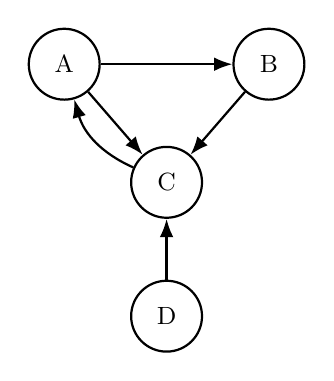
\begin{tikzpicture}[node distance=2.1cm, every node/.style={draw,circle,minimum size=0.9cm,font=\small}, ->,>=Latex,thick]
  \node (A) at (0,1.2) {A};
  \node (B) at (2.6,1.2) {B};
  \node (C) at (1.3,-0.3) {C};
  \node (D) at (1.3,-2.0) {D};
  \draw (A) -- (B);
  \draw (A) -- (C);
  \draw (B) -- (C);
  \draw (C) to[bend left=25] (A);
  \draw (D) -- (C);
\end{tikzpicture}
\end{center}

\textbf{Update equations} (from the inlinks of each page):
\[
PR(A)=0.0375+0.85\,PR(C), \quad PR(B)=0.0375+0.85\,\tfrac{PR(A)}{2}
\]
\[
PR(C)=0.0375+0.85\left(\tfrac{PR(A)}{2}+PR(B)+PR(D)\right), \quad PR(D)=0.0375
\]
($D$ has no inlinks, so its rank is \emph{always} exactly the teleport value -- it never changes across iterations.)

\textbf{Power iteration}, starting from $PR_0(A)=PR_0(B)=PR_0(C)=PR_0(D)=0.25$:

\begin{center}
\begin{tabular}{@{}lcccc@{}}
\toprule
Iteration & $PR(A)$ & $PR(B)$ & $PR(C)$ & $PR(D)$ \\
\midrule
0 & 0.2500 & 0.2500 & 0.2500 & 0.2500 \\
1 & 0.2500 & 0.1438 & 0.5688 & 0.0375 \\
2 & 0.5209 & 0.1438 & 0.2978 & 0.0375 \\
3 & 0.2906 & 0.2589 & 0.4130 & 0.0375 \\
\bottomrule
\end{tabular}
\end{center}

(Sample computation, iteration 2: $PR_2(A)=0.0375+0.85(0.5688)=0.5209$; \ $PR_2(C)=0.0375+0.85\big(\tfrac{0.25}{2}+0.1438+0.0375\big)=0.0375+0.85(0.30625)=0.2978$.) Each row sums to $1$, as required.

\textbf{Exact algebraic solution.} Substituting $PR(D)=0.0375$ and $PR(B)=0.0375+0.425\,PR(A)$ into the $PR(C)$ equation, then into the $PR(A)$ equation, gives a single equation in $PR(A)$:
\[
PR(A) = 0.1235625 + 0.6683125\,PR(A) \ \Longrightarrow\ PR(A) = \frac{0.1235625}{0.3316875} \approx 0.3725
\]
\[
PR(B) = 0.0375+0.425(0.3725)\approx0.1958, \qquad PR(C) = \frac{PR(A)-0.0375}{0.85}\approx0.3941, \qquad PR(D)=0.0375
\]
Check: $0.3725+0.1958+0.3941+0.0375 = 0.9999\approx1$ (rounding). The power-iteration table above is visibly converging toward exactly this vector -- $C$ has the highest rank because it receives inlinks from three different pages ($A$, $B$, and $D$).
\end{examplebox}

\begin{exercisebox}[Practice Exercise 7.2]
Three pages $\{X,Y,Z\}$ with links $X\to Y$, $Y\to Z$, $Z\to X$, $Z\to Y$ (so $L(X)=1, L(Y)=1, L(Z)=2$). Use $d=0.85$, $N=3$.
\begin{enumerate}[label=(\alph*)]
  \item Write the three PageRank update equations.
  \item Starting from $PR_0(X)=PR_0(Y)=PR_0(Z)=\tfrac13$, compute $PR_1$ and $PR_2$ for all three pages.
  \item Set up (you do not need to fully re-derive) the exact linear system and confirm the given answer $PR(X)\approx0.215,\ PR(Y)\approx0.397,\ PR(Z)\approx0.388$ is at least \emph{consistent} with the direction your iterations are moving.
\end{enumerate}
\end{exercisebox}

\Solution
\textbf{(a)} Teleport term $=\dfrac{1-0.85}{3}=0.05$.
\[
PR(X) = 0.05 + 0.425\,PR(Z), \qquad PR(Y) = 0.05 + 0.85\,PR(X) + 0.425\,PR(Z), \qquad PR(Z) = 0.05+0.85\,PR(Y)
\]
\textbf{(b)}
\begin{center}
\begin{tabular}{@{}lccc@{}}
\toprule
Iteration & $PR(X)$ & $PR(Y)$ & $PR(Z)$ \\
\midrule
0 & 0.3333 & 0.3333 & 0.3333 \\
1 & 0.1917 & 0.4750 & 0.3333 \\
2 & 0.1917 & 0.3546 & 0.4538 \\
\bottomrule
\end{tabular}
\end{center}
(e.g., $PR_1(Y) = 0.05+0.85(0.3333)+0.425(0.3333) = 0.05+0.2833+0.1417=0.4750$; $\ PR_2(Z)=0.05+0.85(0.4750)=0.4538$.)\\
\textbf{(c)} After 2 iterations $Y$ is still the largest (as in the target answer) and $Z$ is rising toward its target of $0.388$ while $X$ has already nearly settled near $0.19$--$0.22$; continuing the iteration a few more rounds converges to the stated $(0.215, 0.397, 0.388)$, confirming consistency.

\subsection{HITS: Hubs and Authorities (Brief)}

An alternative link-analysis model computes two scores per page: a \textbf{hub score} (points to many good authorities) and an \textbf{authority score} (is pointed to by many good hubs), updated by mutual reinforcement: $auth(p) \leftarrow \sum_{q\to p} hub(q)$, then $hub(p) \leftarrow \sum_{p \to r} auth(r)$, repeated and renormalized -- unlike PageRank, HITS scores are computed \emph{per query} over the local neighborhood of pages relevant to that query, not once for the whole web.

% ======================================================================
% WEEK 8
% ======================================================================
\weekpart{8}{Course Review and Synthesis}

\section{The Big Picture: How the Models Connect}

Every model in this course answers the same underlying question -- \emph{how relevant is document $d$ to query $q$?} -- with increasing sophistication:

\begin{center}
\begin{tabular}{@{}p{2.6cm}p{5.6cm}p{6.2cm}@{}}
\toprule
\textbf{Model} & \textbf{Core idea} & \textbf{Main limitation it fixes vs.\ the previous model} \\
\midrule
Boolean (Wk 1) & Exact set membership via AND/OR/NOT & -- (baseline) \\
tf-idf / VSM (Wk 3) & Geometric similarity, graded relevance & Boolean gives no ranking at all \\
BM25 (Wk 3) & Saturating tf, document-length normalization & raw tf-idf grows without bound and ignores length \\
BIM / RSJ (Wk 5) & Explicit probability of relevance, from Bayes' rule & VSM has no probabilistic justification \\
Language Models (Wk 5) & Smoothed generative model of text itself & BIM's binary (0/1) term representation loses tf information \\
Na\"ive Bayes (Wk 6) & Same generative machinery, applied to a \emph{labeled class} instead of a query & extends the LM idea to supervised classification \\
PageRank (Wk 7) & Query-independent authority from hyperlink structure & all previous models score \emph{content only}, ignoring the web graph \\
\bottomrule
\end{tabular}
\end{center}

\section{Master Formula Sheet}

\begin{center}
\small
\begin{tabular}{@{}p{3.6cm}p{10.8cm}@{}}
\toprule
\textbf{Concept} & \textbf{Formula} \\
\midrule
Merge cost & $O(x+y)$ \\
$idf$ & $idf_t = \log(N/df_t)$ \\
tf-idf & $tf\text{-}idf_{t,d} = tf_{t,d}\times idf_t$ \\
Cosine similarity & $\cos(\vec q,\vec d) = \dfrac{\vec q\cdot\vec d}{\lVert\vec q\rVert\lVert\vec d\rVert}$ \\
BM25 & $\sum_{t\in Q} idf(t)\dfrac{f(t,D)(k_1+1)}{f(t,D)+k_1(1-b+b|D|/\text{avgdl})}$ \\
Precision / Recall / $F_1$ & $P=\dfrac{TP}{TP+FP}$, $R=\dfrac{TP}{TP+FN}$, $F_1=\dfrac{2PR}{P+R}$ \\
AP / MAP & $AP=\dfrac1R\sum_{\text{rel } d} P(\text{rank of }d)$; $MAP$ = mean of $AP$ over queries \\
DCG / nDCG & $DCG_p=rel_1+\sum_{i=2}^p \dfrac{rel_i}{\log_2 i}$; \ $nDCG_p = DCG_p/IDCG_p$ \\
Rocchio & $\vec q_m = \alpha\vec q_0+\beta\,\overline{D_r}-\gamma\,\overline{D_{nr}}$ \\
RSJ weight & $c_t = \log\dfrac{p_t(1-u_t)}{u_t(1-p_t)}$ \\
Jelinek--Mercer & $P_{JM}(t\mid d) = (1-\lambda)P_{\text{mle}}(t\mid d)+\lambda P(t\mid C)$ \\
Dirichlet smoothing & $P_{\text{Dir}}(t\mid d) = \dfrac{tf_{t,d}+\mu P(t\mid C)}{|d|+\mu}$ \\
Na\"ive Bayes & $c_{\text{map}}=\arg\max_c P(c)\prod_t P(t\mid c)^{tf_{t,d}}$; \ $\hat P(t\mid c)=\dfrac{T_{ct}+1}{\sum_{t'}T_{ct'}+|V|}$ \\
PageRank & $PR(p)=\dfrac{1-d}{N}+d\sum_{q\to p}\dfrac{PR(q)}{L(q)}$ \\
Edit distance & $D[i,j]=\min\big(D[i\text{-}1,j]{+}1,\,D[i,j\text{-}1]{+}1,\,D[i\text{-}1,j\text{-}1]{+}\mathbb{1}[s_1[i]\ne s_2[j]]\big)$ \\
Jaccard coefficient & $J(X,Y) = |X\cap Y| / |X\cup Y|$ \\
\bottomrule
\end{tabular}
\end{center}

\section{Comprehensive Review Problems}

\begin{exercisebox}[Review Problem 8.1 -- Boolean Merge Order (Week 1)]
Document frequencies: $df(\textsf{apple})=800$, $df(\textsf{banana})=50$, $df(\textsf{cherry})=200$. For \textsf{apple AND banana AND cherry}, give the optimal merge order and an upper bound on the total number of comparisons.
\end{exercisebox}
\Solution
Order by increasing $df$: \textsf{banana} (50), \textsf{cherry} (200), \textsf{apple} (800). Merge \textsf{banana} and \textsf{cherry} first (cost $\le 50+200=250$, result $\le50$ items), then merge that result with \textsf{apple} (cost $\le 50+800=850$). Total $\le 1100$ comparisons -- far less than merging \textsf{apple} and \textsf{cherry} first ($\le 800+200=1000$ for that single step alone).

\begin{exercisebox}[Review Problem 8.2 -- Edit Distance (Week 2)]
Compute the edit distance between \textsf{pearl} and \textsf{earl}.
\end{exercisebox}
\Solution
$\textsf{earl}$ is obtained from $\textsf{pearl}$ by deleting the leading \textsf{p}. Edit distance $=1$.

\begin{exercisebox}[Review Problem 8.3 -- tf-idf and Cosine Similarity (Week 3)]
$N=4$. $df(x)=4$ (so $idf_x=\log_2(4/4)=0$), $df(y)=2$ ($idf_y=\log_2(4/2)=1$), $df(z)=1$ ($idf_z=\log_2(4/1)=2$). Document $E$ has $tf(x)=6,tf(y)=3,tf(z)=2$. Query $=$ ``$y\ z$'', giving $Q=(0,1,2)$ in $idf$-weighted form. Compute $\cos(Q,E)$.
\end{exercisebox}
\Solution
$E = (6\times0,\,3\times1,\,2\times2) = (0,3,4)$. $\lVert E\rVert=\sqrt{9+16}=5$. $\lVert Q\rVert=\sqrt{1+4}=\sqrt5\approx2.236$. $Q\cdot E = 1(3)+2(4)=11$.
\[
\cos(Q,E) = \frac{11}{5\times2.236} = \frac{11}{11.18} \approx 0.984
\]

\begin{exercisebox}[Review Problem 8.4 -- BM25 (Week 3)]
$N=5$, $df(t)=1$ so $idf(t)=\ln\frac{5-1+0.5}{1+0.5}=\ln 3\approx1.0986$. $\text{avgdl}=20$, $k_1=1.2$, $b=0.75$. Document $D$ has $|D|=20$ (exactly average) and $f(t,D)=2$. Compute $\text{score}(D,\{t\})$.
\end{exercisebox}
\Solution
Since $|D|=\text{avgdl}$, the length factor is exactly $1-b+b(1)=1$, so the denominator is simply $f(t,D)+k_1 = 2+1.2=3.2$.
\[
\text{score} = 1.0986\times\frac{2(2.2)}{3.2} = 1.0986\times\frac{4.4}{3.2} = 1.0986\times1.375 \approx 1.511
\]

\begin{exercisebox}[Review Problem 8.5 -- Precision, Recall, $F_1$ (Week 4)]
$15$ documents are relevant to a query. A system retrieves $10$ documents, of which $7$ are relevant. Compute $P$, $R$, $F_1$.
\end{exercisebox}
\Solution
$TP=7,FP=3,FN=8$. $P=7/10=0.7$, $R=7/15\approx0.467$.
\[
F_1 = \frac{2(0.7)(0.467)}{0.7+0.467} = \frac{0.653}{1.167} \approx 0.560
\]

\begin{exercisebox}[Review Problem 8.6 -- nDCG (Week 4)]
Ranked relevance $rel=[1,2,0,3]$. Compute $DCG_4$, $IDCG_4$, $nDCG_4$.
\end{exercisebox}
\Solution
$DCG_4 = 1+\dfrac{2}{\log_22}+\dfrac{0}{\log_23}+\dfrac{3}{\log_24} = 1+2+0+1.5=4.5$.\\
Ideal order $[3,2,1,0]$: $IDCG_4 = 3+\dfrac{2}{1}+\dfrac{1}{1.585}+\dfrac{0}{2} = 3+2+0.631+0=5.631$.
\[
nDCG_4 = \frac{4.5}{5.631} \approx 0.799
\]

\begin{exercisebox}[Review Problem 8.7 -- Rocchio (Week 4)]
$\vec q_0=(1,1)$, one relevant document $\vec d=(2,0)$, one non-relevant document $\vec d\,'=(0,2)$. Using $\alpha=1,\beta=0.75,\gamma=0.25$, compute $\vec q_m$.
\end{exercisebox}
\Solution
\[
\vec q_m = (1,1) + 0.75(2,0) - 0.25(0,2) = (1,1)+(1.5,0)-(0,0.5) = (2.5,\ 0.5)
\]

\begin{exercisebox}[Review Problem 8.8 -- Na\"ive Bayes (Week 6)]
Training: \textbf{Fruit} docs -- ``sweet red apple'', ``sweet orange citrus''; \textbf{Vegetable} docs -- ``green leafy spinach'', ``green bitter kale''. Test: ``sweet green apple''. $|V|=10$. Classify using add-one smoothing.
\end{exercisebox}
\Solution
$N=4$, $N_{\text{Fruit}}=N_{\text{Veg}}=2 \Rightarrow \hat P(\text{Fruit})=\hat P(\text{Veg})=0.5$. Fruit counts (total $6$): sweet$=2$, apple$=1$, green$=0$. Vegetable counts (total $6$): green$=2$, sweet$=0$, apple$=0$.
\[
\hat P(\textsf{sweet}\mid F)=\tfrac{3}{16},\ \hat P(\textsf{green}\mid F)=\tfrac{1}{16},\ \hat P(\textsf{apple}\mid F)=\tfrac{2}{16}
\]
\[
\hat P(\textsf{sweet}\mid V)=\tfrac{1}{16},\ \hat P(\textsf{green}\mid V)=\tfrac{3}{16},\ \hat P(\textsf{apple}\mid V)=\tfrac{1}{16}
\]
\[
\text{Score}(F) = 0.5\times\tfrac{3}{16}\times\tfrac{1}{16}\times\tfrac{2}{16} \approx 7.32\times10^{-4}, \qquad
\text{Score}(V) = 0.5\times\tfrac{1}{16}\times\tfrac{3}{16}\times\tfrac{1}{16} \approx 3.66\times10^{-4}
\]
$\text{Score}(F)$ is exactly twice $\text{Score}(V)$ (both share the factor $\tfrac{3}{16}\times\tfrac1{16}$; the remaining factors are $\tfrac{2}{16}$ vs.\ $\tfrac1{16}$) $\Rightarrow$ classify as \textbf{Fruit}.

\begin{exercisebox}[Review Problem 8.9 -- PageRank on a Symmetric Cycle (Week 7)]
Three pages $P\to Q\to R\to P$ (a pure cycle, each page has exactly one outlink and one inlink). Using $d=0.85$, starting from $PR_0=\tfrac13$ for all three pages, compute $PR_1$ for each page. What do you notice, and why does it happen?
\end{exercisebox}
\Solution
Teleport term $=\frac{0.15}{3}=0.05$. Every page has exactly one inlink from a page with rank $\tfrac13$ and out-degree $1$:
\[
PR_1(P) = 0.05 + 0.85\times\frac13 = 0.05+0.2833 = 0.3333 = \frac13
\]
By the same computation, $PR_1(Q)=PR_1(R)=\tfrac13$ too -- \textbf{the distribution does not change}. This is because a symmetric cycle is already at its stationary distribution: every page has exactly one inlink carrying exactly the same rank as every other page, so the uniform distribution is a fixed point of Key Formula 7.1.

% ======================================================================
% APPENDIX
% ======================================================================
\clearpage
\phantomsection
\addcontentsline{toc}{part}{Appendix}
\begin{center}
\rule{0.9\textwidth}{1pt}\\[4pt]
{\Huge\bfseries\color{primary} Appendix}\\[4pt]
\rule{0.9\textwidth}{1pt}
\end{center}
\vspace{1em}

\section*{Further Reading}
\addcontentsline{toc}{section}{Further Reading}

\textbf{Primary text (all weeks):} Manning, C. D., Raghavan, P., \& Sch\"utze, H. (2009). \textit{An Introduction to Information Retrieval}. Cambridge University Press. Freely available at \url{http://www.informationretrieval.org/}.

\begin{itemize}
  \item \textbf{Week 1:} Waller, W. G., \& Kraft, D. H. (1979). A mathematical model of a weighted Boolean retrieval system. \textit{Information Processing \& Management}, 15(5), 235--245.
  \item \textbf{Week 3:} Lee, D. L., Chuang, H., \& Seamons, K. (1997). Document ranking and the vector-space model. \textit{IEEE Software}, 14(2), 67--75. \quad Ramos, J. (2003). Using tf-idf to determine word relevance in document queries. \textit{Proceedings of the First Instructional Conference on Machine Learning}, 242(1), 29--48.
  \item \textbf{Week 4:} Bama, S. S., Ahmed, M. I., \& Saravanan, A. (2015). A survey on performance evaluation measures for information retrieval systems. \textit{International Research Journal of Engineering and Technology}, 2(2), 1015--1020. \quad Lavrenko, V., \& Croft, W. B. (2017). Relevance-based language models. \textit{ACM SIGIR Forum}, 51(2), 260--267.
  \item \textbf{Week 7:} Bharat, K., \& Broder, A. (1998). A technique for measuring the relative size and overlap of public web search engines. \textit{Computer Networks and ISDN Systems}, 30(1--7), 379--388. (The source of the index-overlap technique in Worked Example 7.1.)
\end{itemize}

\section*{Notation Glossary}
\addcontentsline{toc}{section}{Notation Glossary}

\begin{center}
\begin{tabular}{@{}lp{11.5cm}@{}}
\toprule
Symbol & Meaning \\
\midrule
$N$ & Number of documents in the collection \\
$V$ & Vocabulary (set of distinct terms); $|V|$ its size \\
$df_t$ & Document frequency of term $t$ (\# documents containing $t$) \\
$tf_{t,d}$ & Term frequency of $t$ in document $d$ \\
$idf_t$ & Inverse document frequency of $t$ \\
$\vec d,\vec q$ & tf-idf vector representations of a document / query \\
$R$ & (Week 4/5) total number of documents relevant to a query \\
$P(c)$ & Prior probability of class $c$ \\
$P(t\mid c)$ & Probability of term $t$ given class/model $c$ \\
$PR(p)$ & PageRank score of page $p$ \\
$L(q)$ & Out-degree (number of outgoing links) of page $q$ \\
$d$ & (Week 7 only) PageRank damping factor \\
\bottomrule
\end{tabular}
\end{center}

\end{document}
